\chapter{Control for \SB{} Locomotion}
\label{controls}

\section{Basic Locomotion Concepts for a Icosahedron Tensegrity Robot}
\label{basic_locomotion}

Locomotion for tensegrity structures like \SB{} is achieved by deforming the structure in a way in which moves the system's center of mass to an unstable configuration, tipping the robot over.
This deformation is usually achieved by either changing the length of the main cable network on the outside of the robot~\cite{sabelhaus2015system,kim2014rapid} or by adding additional cables which run through the structure connecting non-parallel rods~\cite{caluwaerts2014design}.
For the rest of this section, deformation is assumed to be done by actuating the main cable network on the outside of the robot since this is how \SB{} is deformed.

\begin{figure}[thpb]
      \centering
      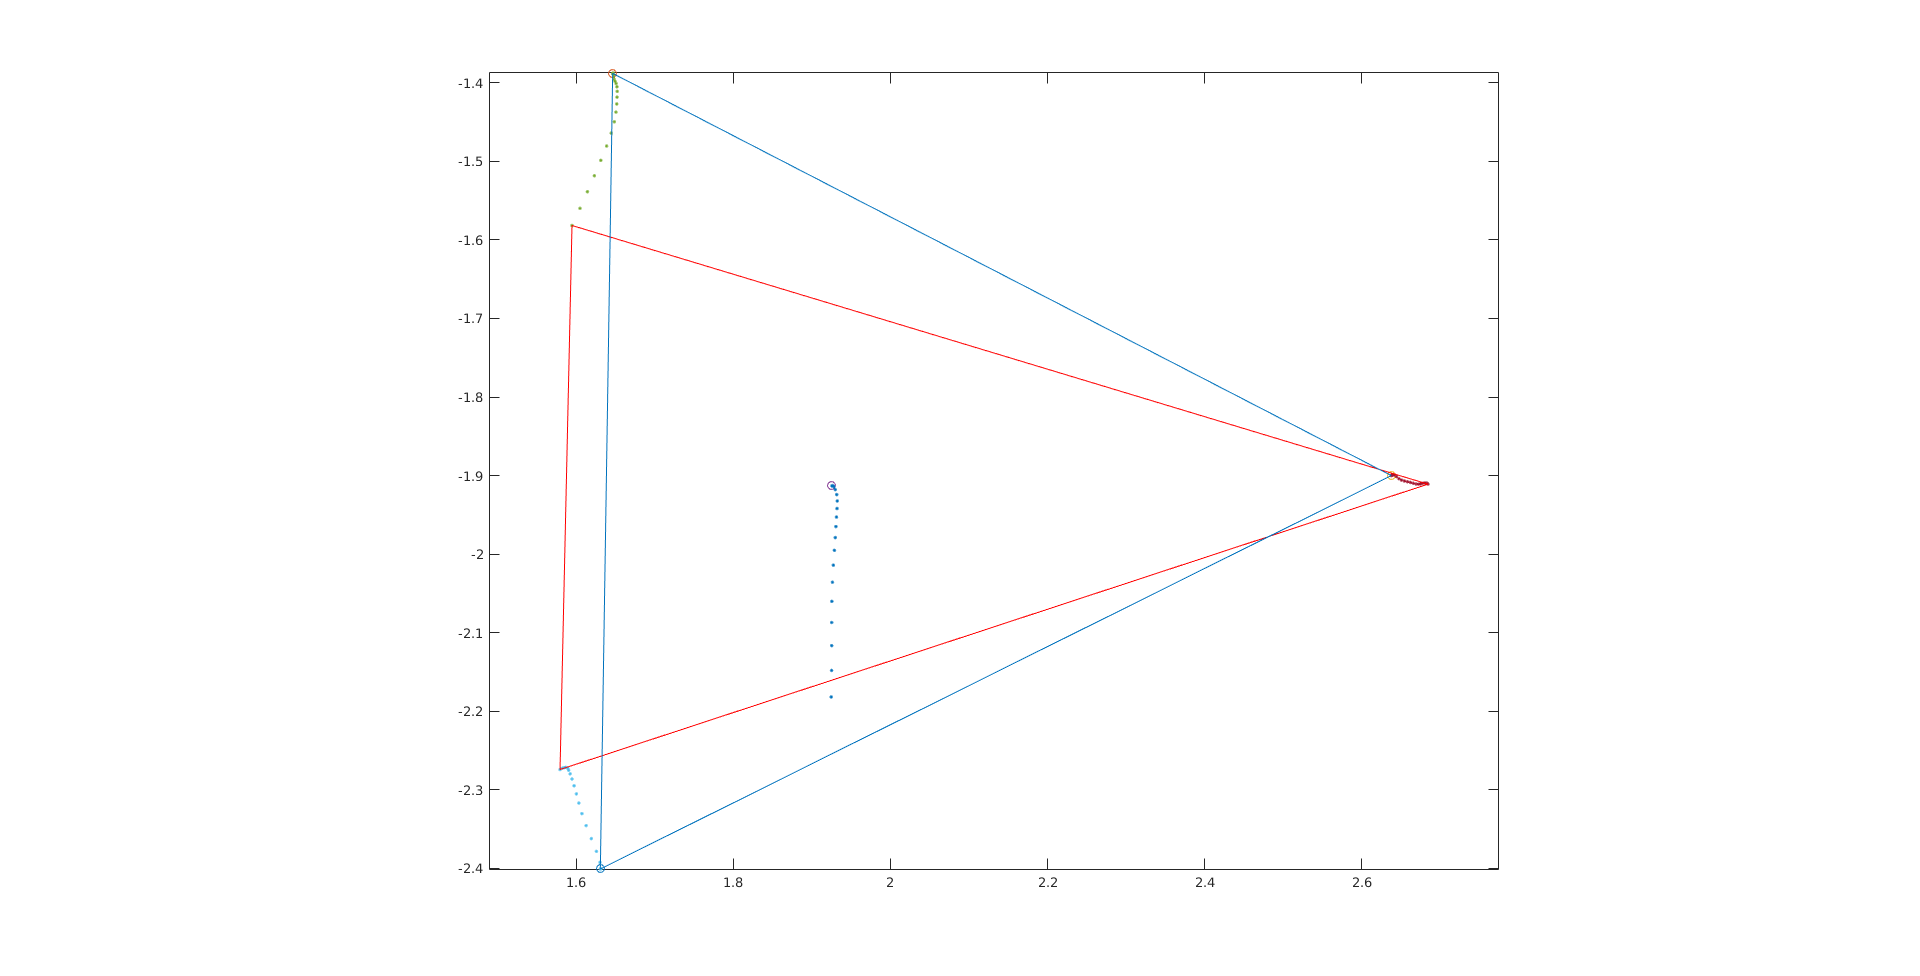
\includegraphics[width=1\columnwidth]{tex/img/Single_flop_bottom_triangle}
      \caption{This is XY data of the bottom triangle of a NTRT simulation of \SB{} performing a single face transition by changing only one side of the bottom triangle.
      No other cable on the system is being actuated during this simulation.
      The blue triangle is the bottom triangle at the start of the simulation. 
      The centralized circle represents the center of mass (CoM) of the entire simulated \SB{} and the dots represents how the CoM moves through time. 
      The red triangle is the configuration where the CoM moves out of the bottom triangle and the robot begins to transition to another face.
      Thus, under ideal conditions and actuation limits, a \SB{} like structure can perform a face transition by the changing of a single cable.}
      \label{fig:single_flop}
\end{figure}

% \SB{} is a tensegrity structure is the shape of an icosahedron.
An regular convex icosahedron is a geometric shape consisting of eight equilateral triangle interlaced with twelve isosceles triangles.
In a passively sable configuration, the bottom of an icosahedron will be resting on either an equilateral or a isosceles triangle.
Utilizing this knowledge, the most simple method for moving the center of mass of an icosahedron can be obtained by changing the length of one side of the bottom triangle to near zero.
This will always move the center of mass to an unstable configuration by effectively reducing the bottom triangle, as seen if figure~\ref{fig:single_flop}, which will cause the robot to transition to another face.
However, this simple control method is not always obtainable on a real robotic system due to limitation on actuation or design methodology.
For \SB{}, this control method is obtainable when the system only has the battery mounted required to actuate the single motor reducing the overall system weight.
Figure~\ref{fig:superball_flop_flat} shows this single motor face transition on a weight reduced \SB{}.

\begin{figure}[thbp]
    \centering
    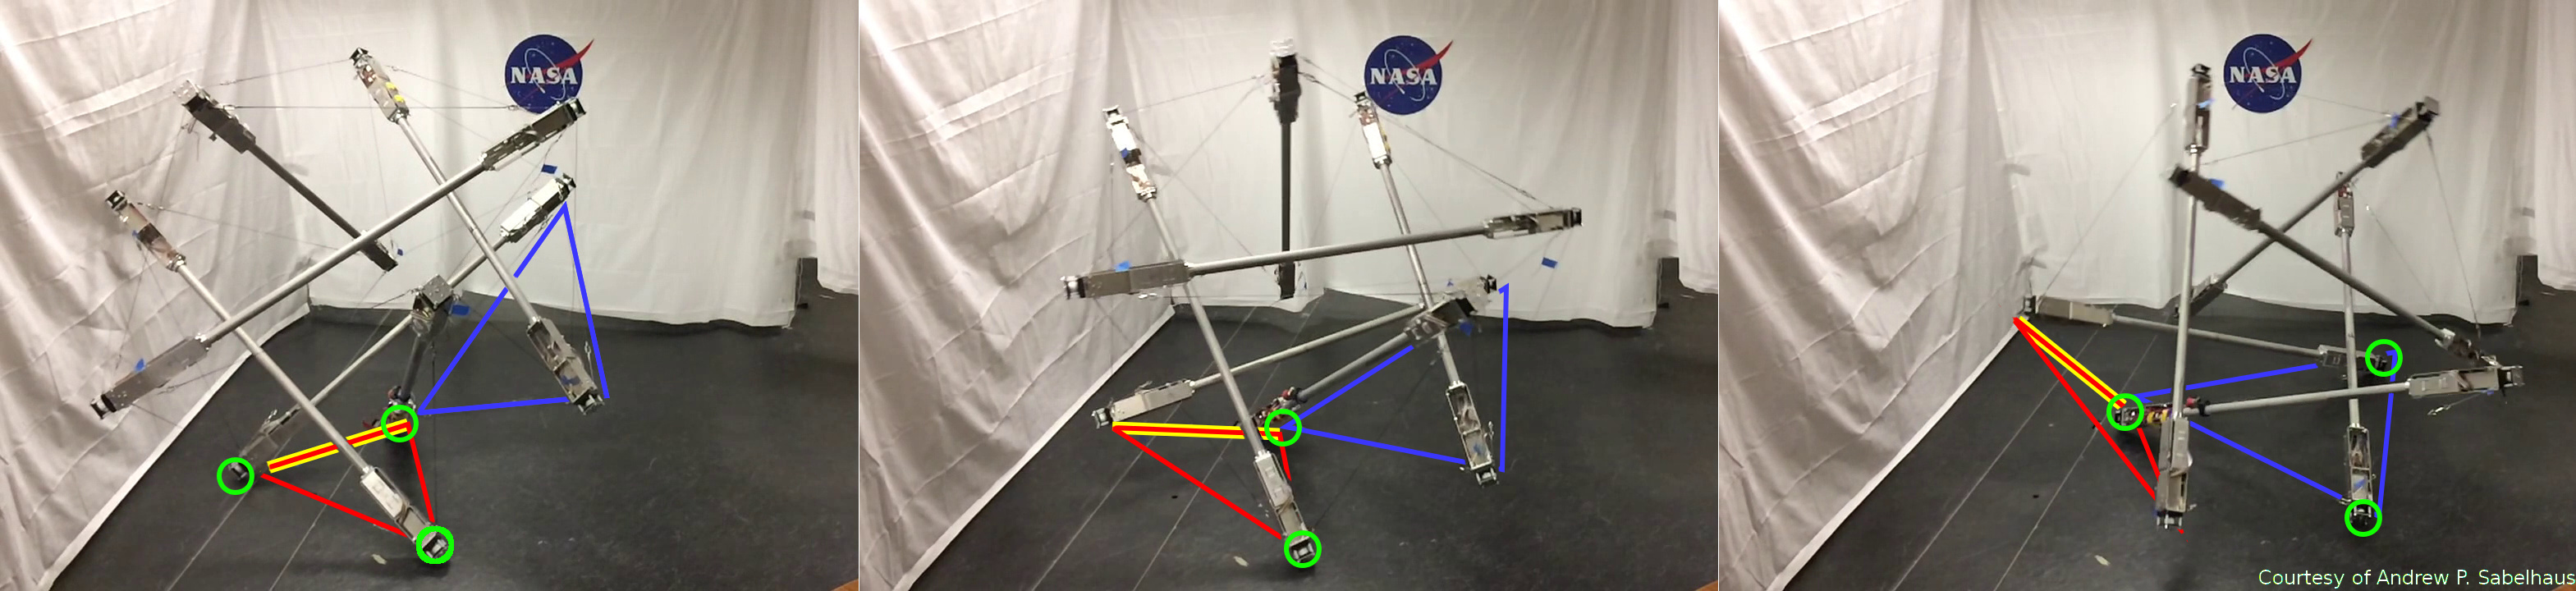
\includegraphics[width=1\linewidth]{tex/img/superball_flop_combined_betterlabels}
    \caption{\SB{} performing a single face-change movement, from one equilateral triangular face to another. The robot begins with all MTRs of the red triangle touching the ground. Then, \SB{} retracts the yellow-highlighted cable on the red triangle, inducing movement. Frame 2 shows \SB{} halfway through the movement with only two points of contact on the ground. Finally, frame 3 shows \SB{} at the end, with all 3 points of the blue triangle in ground contact.}
    \label{fig:superball_flop_flat}
\end{figure}

\subsection{\SB{} Acutation Pattern}
\label{sec:pattern}
\SB{} is an underactuated icosahedron tensegrity robot.
Of the 24 connection cables, \SB{} only has 12 cables which are actively actuated and the other cables are passive as discussed in section~\ref{design}.
Since each MTR is manufactured with the same elements, each of the four cables attached to it are one of four types: an actuated cable attached to a motor, an actuated cable from an adjacent MTR terminating at this MTR, a passive cable attached to a spring, or a passive cable from an adjacent MTR terminating at this MTR.
Therefore, there is a unique pattern of cables, and care is needed when choosing this pattern for locomotion. 

\begin{figure}[thbp]
    \centering
    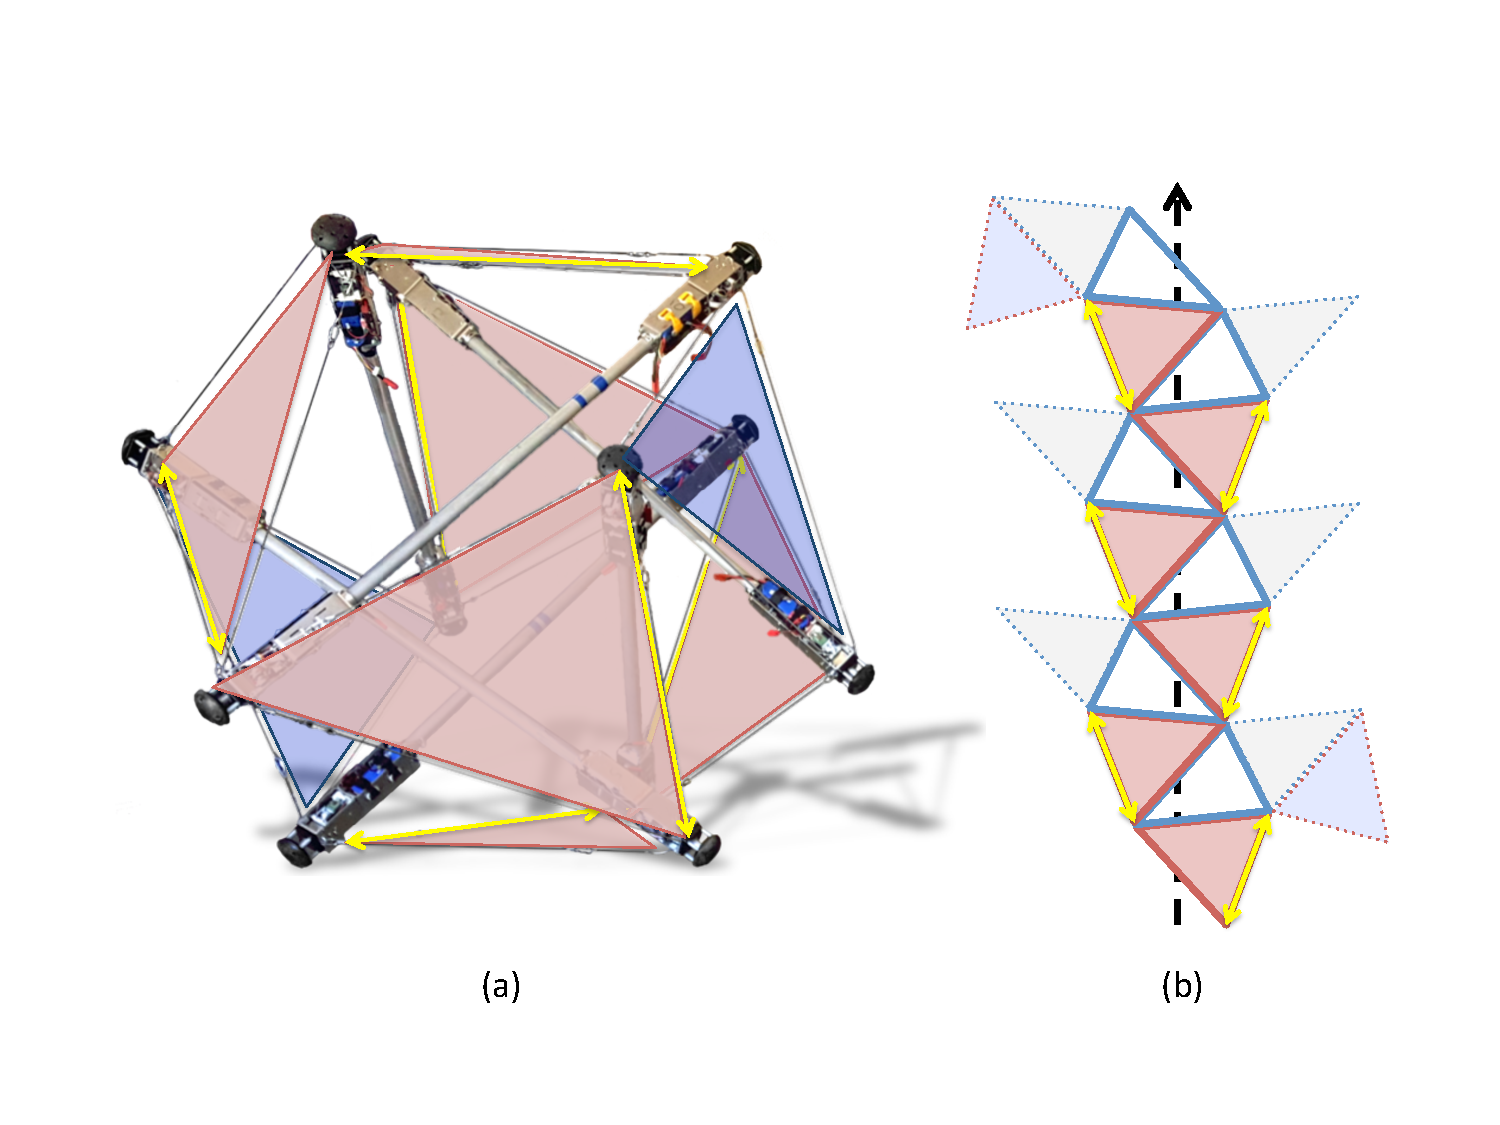
\includegraphics[width=0.8\linewidth]{tex/img/SB_RedvBlue_with_Walk}
    \caption{This image shows the actuation pattern used on \SB{}. There are 8 equilateral triangles, shown in either red or blue. Each red triangle represents a face with only one of the three cable sides actuated. These actuated cables are noted by the yellow double arrows. Each blue triangle, which are not  has actuators on all three cable sides. The basic forward rolling of \SB{} has the robot landing with a red triangle fully on the ground during locomotion. Blue triangles don't touch the ground during this forward rolling pattern. Figure (a) shows each triangle highlighted on \SB{} and figure (b) shows the forward locomotion pattern, or walking pattern, of \SB{}.}
    \label{fig:actuator_pattern}
\end{figure}

For \SB{}, a symmetric pattern is used where each equilateral triangle has at least one actuator associated with one of its sides.
As stated in section~\ref{design}, \SB{} has eight equilateral triangles, so at most three triangles will have more than one actuated side.
These triangles are evenly spaced round the surface of the robot such that there are "rings" of six equilateral triangles with the other two triangles flanking this ring.
Forward locomotion is then achieved by transitioning the structure such that each of the six equilateral triangles on this "ring" come in complete contact with the ground at some instantaneous point in time.
Since a symmetric pattern was desired, it was chosen to placing one actuator per "ring" triangle in such a way where the theoretical full actuation length change of that triangle side would cause the robot to transition towards the next sequential equilateral triangle on that "ring".
The other six motors where then attached as all the side of the remaining two equilateral triangles, those not associated with the "ring".
Figure~\ref{fig:actuator_pattern} (a) shows a graphical overlay of the actuation "ring" and the fully actuated triangles marked in red and blue, respectively.
Figure~\ref{fig:actuator_pattern} (b) is a icosahedron rolled out to show the "walking" gait pattern achieved by rolling about the actuation "ring".

\subsection{Basic Steering Controller}
\label{sec:steering}
THe majority of this chapter deals with how to achieve a continuous forward locomotion gait for \SB{}.
However, having the ability to turn makes navigation a bit more interesting and this section will discuss some preliminary results in achieving a simple left and right turning gait.
It has been shown in literature that a simulated fully actuated (24 actuators) \SB{} like robot can achieve left and right turning gaits~\cite{kim2014rapid} as well as goal direction navigation~\cite{iscen2014flop}.

The current version of \SB{} has limited actuation as stated in section~\ref{basic_locomotion} and can not perform the published turning gaits.
A simple solution which can be implemented with any type of forward locomotion controller involves the use of the two fully actuated equilateral triangles outlined in section~\ref{sec:pattern} and shown in figure~\ref{fig:actuator_pattern}.
Actuating all three motors for a given triangle equal amounts (squeezing) biases the gait such that the roll performs a wide turn.
Squeezing the triangle on the left side biases the robot left, and conversely squeezing the right triangle biases the robot right.
This behavior can be seen in figure~\ref{fig:turning}.

\begin{figure}[thbp]
    \centering
    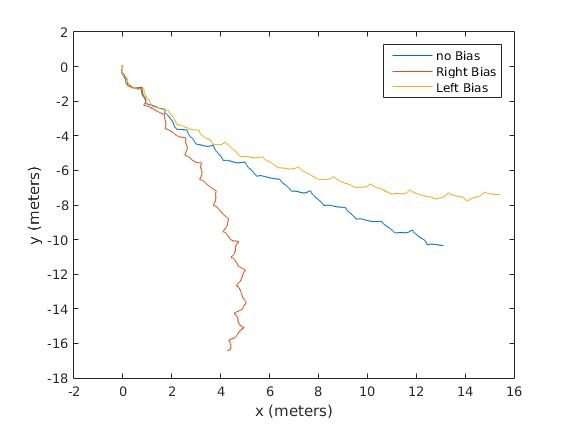
\includegraphics[width=0.8\linewidth]{tex/img/left_right_paths}
    \caption{}
    \label{fig:turning}
\end{figure}

\section{Hand-Tuned Stepwise Controller}
\label{hand_stepwise}
The initial controller developed for \SB{} was a basic open loop, hand tuned controller.
Motor position commands where systematically found through experimentation which moved the robot into a kinematically unstable configuration for each of the six faces mentioned in section~\ref{basic_locomotion}.
Under normal conditions on flat ground, when the system starts on an equilateral triangle the forward momentum of the structure after deformation will push it through the isosceles triangle and come to rest on another equilateral triangle.
Using this assumption, only six different kinematic configurations where implemented.
To automate this process, enabling the system to detect which face it resided on was necessary.
A simple K-nearest neighbor algorithm was implemented on recorded IMU data for each equilateral triangle face of \SB{}.
Since the faces are discrete enough, one hundred percent classification was found.
With this information, a basic open loop controller was written that used the detected face as an input and commanded the correct motor commands for the kinematically unstable configuration to transition the robot to the next face.

\begin{figure}[thpb]
      \centering
      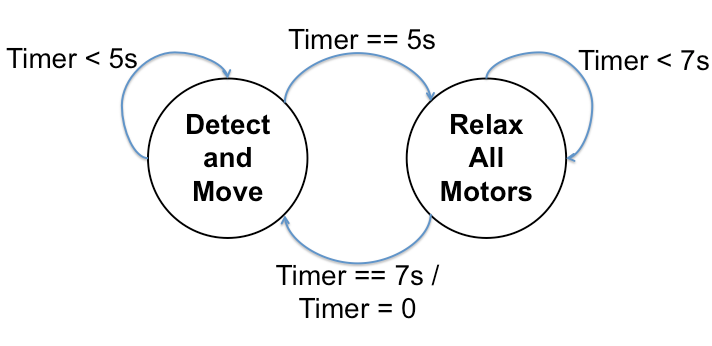
\includegraphics[width=0.7\columnwidth]{tex/img/Stepwise_state_machine/Slide1_fixed}
      \caption{Time based state machine which automates the hand-tuned stepwise controller. Timers are used to allow for dynamic settling before the next action is taken.}
      \label{fig:stepwise_fsm}
\end{figure}

Once the robot acted the kinematically unstable configuration, all motor commands were set back to their starting configuration.
This ensured correct detection and transition time for the next cycle.
The hand-tuned stepwise controller has two main states, a detect and move state and a relax state as seen in~\ref{fig:stepwise_fsm}.
The transition between each state is time based, where the timing between states was empirically obtained to ensure transition and dynamic settling.
It should be noted that for \SB{}, a single face transition requires more than the single motor command as stated in section~\ref{basic_locomotion}.
This non ideal behavior is caused by many factors, but a major factor is the maximum tension a single cable should experience during actuation.

\section{Machine Learning Enabled Controllers}
\label{sec:machine_learning}
The previous sections in this chapter dealt with locomotion controllers that are idealistically simple as in section~\ref{basic_locomotion} or completely derived by human experimentation as in section~\ref{hand_stepwise}.
Thus, these controllers do not leverage any inherent properties within the tenesgrity structure or have the ability to optimize around any limitations in the structure's design.
One property that will be leveraged in the following sections is global force distribution.
Figure~\ref{fig:nonlinear} shows how the tensioning on a single cable affects all other cables on \SB{}.

\begin{figure}[thpb]
\centering
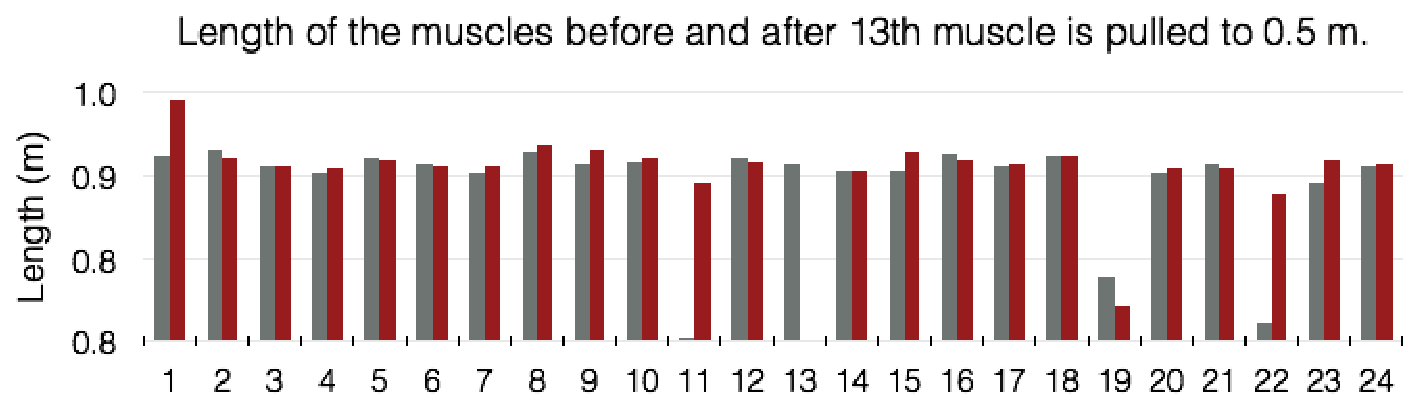
\includegraphics[width=\columnwidth]{tex/ASME-journal/results/actuate1/actuate1.eps}
\caption{Change in length of cables when one (13th) is pulled to 0.5 meters while the others are keep at the same rest length.  Grey bars show original length, red show final length. While the robot is at the exact same orientation, the actual lengths of the cables change in a non-linear way.  Some of the cables shorten due to the tension introduced by cable 13, and some of the cables relax.}
\label{fig:nonlinear}
\end{figure}

The majority of the learned controllers discussed in this section will be implemented in the NTRT simulation environment with the final locomotion controller implemented on the \SB{} hardware.
The first section will discuss a two stage Monte Carlo method for maneuvering \SB{} out of craters/holes.
This if followed by an open loops learned controller for forward navigation.
Finally, the last section discusses a closed loop locomotion controller developed in simulation and implemented on the physical \SB{} hardware.

% \section{Other Learned Locomotion Behaviors}
% \label{sec:otherControllers}
% Along side the basic forward locomotion controllers discussed above, other locomotion controllers which enable specific tasks are being developed for \SB{} like tensegrity structures.
% A path planning controller based on belief spaces was discussed in section~\ref{sec:belief} of chapter~\ref{chapter:litReview}.
% In this section, an early stage controller for escaping crater like scenarios will be shown which was developed in collaboration with Steve Lessard~\cite{lessard2015robust}.
% Also briefly discussed is an early method on how to steer with the locomotion policy developed in section~\ref{sec:mdgps}.
%In the following sections, two controllers in early stages of their research are shown, one for escaping crater like scenarios and one for high level path planning.
%These were conducted in collaboration with Steve Lessard~\cite{lessard2015robust} and Zakary Littlefield~\cite{littlefieldintegrating}, respectively. 

\subsection{Crater Escape Controller}
\label{sec:crater}
When designing and promoting your system as a more robust solution than current planetary rovers, there come a time in which you need to show that your system has the ability to handle scenarios which were not planned, one simple example could be getting stuck in a hole/crater.
In order to achieve a solution to this task, a two stage Monte Carlo technique is used on a simplified control space on a simulated fully actuated \SB{} in NTRT.
The simplified control space consists of clustering each equilateral triangle, shown in section~\ref{basic_locomotion}, such that all three actuators in that cluster follow a sine wave dictated by equation~\ref{sine}

\begin{align}
y = Asin(\omega t + \varphi) + D
\label{sine}
\end{align}

Where \(A\) is amplitude, \(\omega\) is angular frequency, \(\varphi\) is phase change, and \(D\) is the DC offset.
This makes \(32\) parameters for a policy to learn and search over (\(4 \text{parameters} \time 8 \text{clusters}\).
A successful policy is one where the robot moves a linear distance greater than the maximum radius of the hole/crater it starts in.

There are two stages to this process, where the first stage run \(1000\) samples with evenly distributed random parameters for each sample (generation 0).
The second stage (generation 1) filters out the successful sample from the first stage and runs \(10\) evenly distributed samples around each of the previously successful parameters such that each value is no more than \(\pm 0.05\%\)
Each sample is let run for a simulation time of \(\SI{60}{\second}\).
This approach makes it feasible to run this simulation process in a relatively short time frame (less than 40 minutes on a 2014 or later quad core i7 or equivalent processor), enabling the system to learn a new policy based on a real time estimate of its current state.
It should be noted that this is a simplified open loop control policy of the one used in the open loop locomotion controller found in section~\ref{sec:openLoopControl}.

\subsubsection{Experiment and Results}
Since NTRT is a numerical solver, stability issues can arise when using small numbers.
To mitigate this, all values inside the simulator were increased by a factor of \(100\), e.g. \SB{}'s rod length increase from \(\SI{1.75}{\meter} \text{to} \SI{175}{\meter}\) and the hole/crater is increased from \(\SI{0.5}{\meter} \text{to} \SI{50}{\meter}\).
Following the escape criterion set in the previous section, the robot escapes the hole/creater when a linear distance of \(\SI{25}{meter}\) is reached in the simulation environment.

\begin{figure}[thpb]
\centering
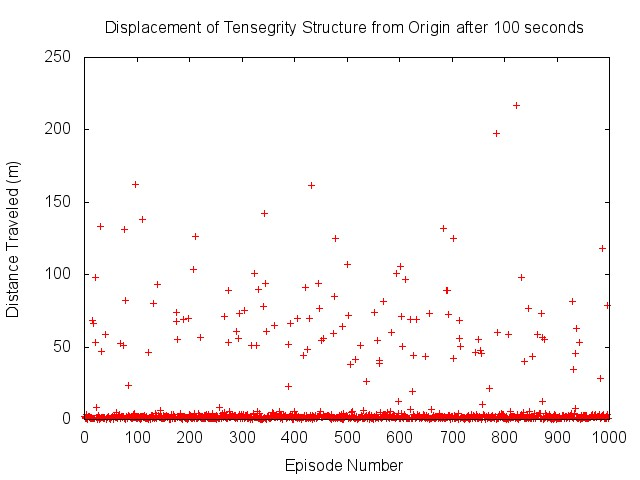
\includegraphics[width=0.8\textwidth]{tex/ARMS_2015/Pictures/gen0distances.jpg}
\caption{Generation 0}
\label{gen0scatter}
\caption{Generations 0 for the escape hole/crater policy. The displacements reached in 1000 independent samples using Monte Carlo generated control policies.}
\end{figure}

\begin{figure}[thpb]
\centering
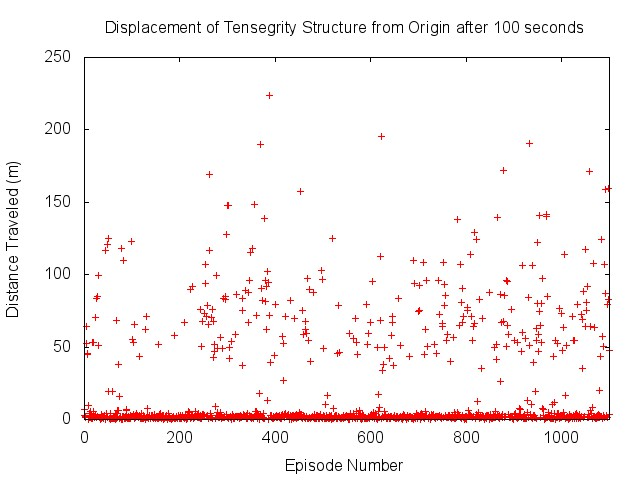
\includegraphics[width=0.8\textwidth]{tex/ARMS_2015/Pictures/gen1distances.jpg}
\caption{Generation 1}
\label{gen1scatter}
\caption{Generations 1 for the escape hole/crater policy. The displacements reached in 1100 independent samples using control policies dictated by the successful samples from Generation 0. The values in the set of sine wave parameters from Generation 1 samples were each centered around one of the successful corresponding sine wave parameters in Generation 0 control policies. These Generation 1 values were then modified to be within 0.5\% of their respective Generation 0 values with the goal of optimizing Generation 0 control policies.}
\end{figure}

Figure~\ref{gen0scatter} shows the simulated robot's CoM displacement for each of the \(1000\) samples in generation 0 of the learning process.
This generation had \(110\) samples which reached a distance of \(\SI{25}{meters}\) or greater.
For generation 1, \(1100\) samples were taken, and its results are shown in figure~\ref{gen1scatter}.

To further explore this policy, a simple comparison is conducted to evaluate how well the policy controls the robot out of a hole/crater with only \(12\) usable actuators.
As a control, \(100\) samples are taken with all actuators functioning, shown in figure~\ref{robust24scatter}.
Then another set of \(100\) samples are taken where only 12 of the actuators are responding to the sine wave command, shown in figure~\ref{robust12scatter}.
The other actuators are modeled as passive linear springs.

\begin{figure}[thpb]
\centering
{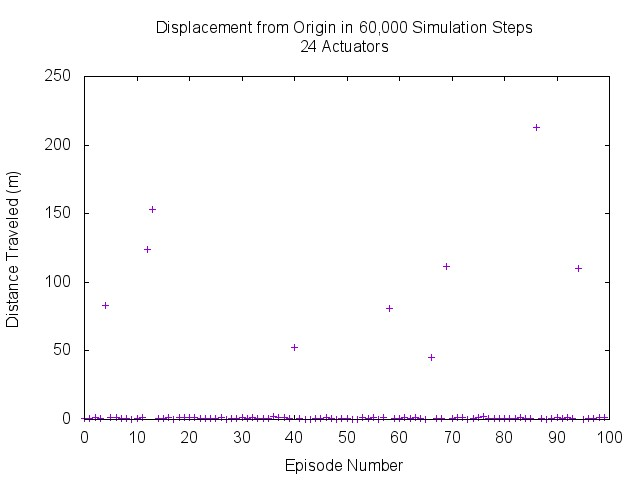
\includegraphics[width=0.8\linewidth]{tex/ARMS_2015/Pictures/dists100.jpg}} 
\caption{100 Samples of Tensegrity Structures with 24 Actuators. By reducing the number of functioning actuators on our simulated tensegrity, the limitations of tensegrity escape can be better explored.
With all 24 actuators on the tensegrity functioning correctly, a successful escape is relatively easy ($9\%$ success rate).}
\label{robust24scatter}
\end{figure}
                       
\begin{figure}[thpb]
\centering
{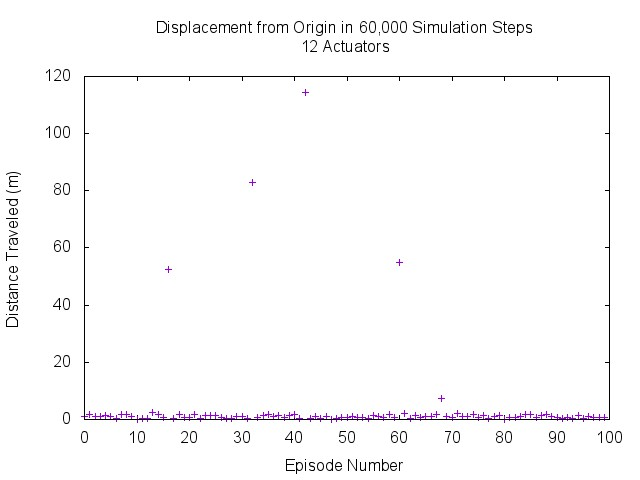
\includegraphics[width=0.8\linewidth]{tex/ARMS_2015/Pictures/dists50.jpg}} 
\caption{100 Samples of Tensegrity Structures with 12 Actuators. With just half of the original actuators functioning correctly, a successful escape is even more difficult (see Figure $7$).
In this generation, $4\%$ of tensegrity rovers were still able to escape the ditch in the allotted time.}
\label{robust12scatter}
\end{figure}

The result of this policy only showed limited success with the second generation only achieving \(24\%\) success.
However, the policy is still able to achieve success even when half of the actuators are turned off.
These preliminary results demonstrate that it is possible to actuate a \SB{} like system out of hole/craters it may be stuck within.

\subsection{Co-Evolutionary Learning for an Open Loop Controller}
\label{sec:openLoopControl}
This section explores an evolutionary controller on a fully actuated (24 actuators) \SB{} like robot, and all the results are based on a simulated robot in NTRT.
However, this work shows how a controller learned through machine learning can utilize the dynamics of such a structure to find optimally consistent locomotion gaits for goal directed behavior.
The work presented in this section are summarized sections of collaborative work found in Iscen~\etal's work~\cite{iscen2015learning}.

% Controlling a tensegrity robot brings multiple challenges such as distributed controls, nonlinear interactions between components and handling difficult to model dynamics such as oscillations. 
% % For this reason traditional centralized controllers and centralized designs are not a good match for a tensegrity robot. 
% In contrast WE present a decidedly distributed approach for controlling a tensegrity robot. 
% On the hardware side, the core of OUR design is an independently controllable rod containing two independent ``end-cap'' controllers on each side of the rod. This model naturally matches the distributed yet holistic nature of a tensegrity. The controllers act independently of each other but they interact through the system, where changing lengths of one of the MUSCLES affects the whole structure in a non-linear way. This behavior can be seen in Figure
% \ref{fig:nonlinear}. When WE pull only one of the MUSCLES (muscle 13), all the MUSCLES change their length while some of them get shorter and some of them get longer. 

% \begin{figure}[t]
% \centering
% 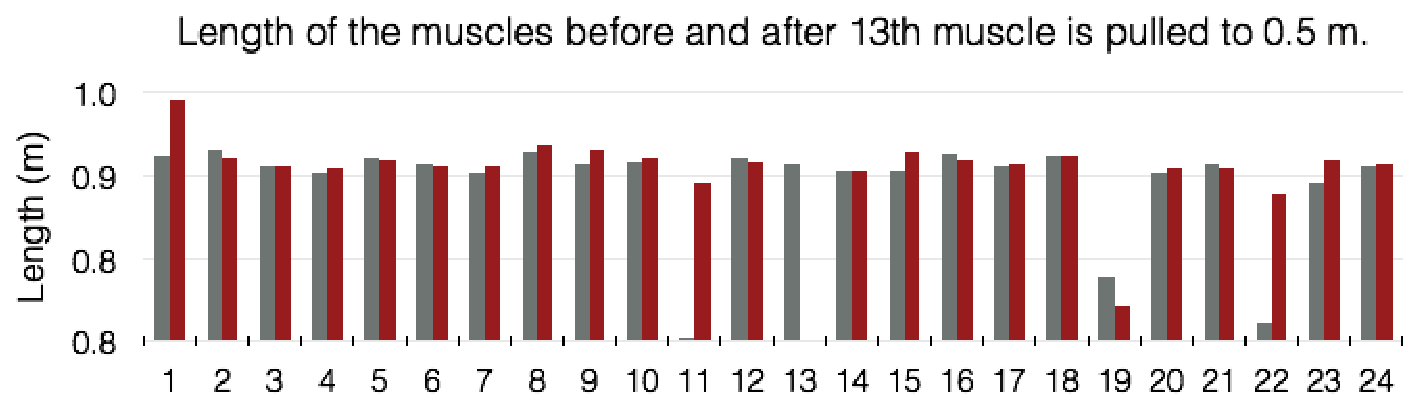
\includegraphics[width=\columnwidth]{tex/ASME-journal/results/actuate1/actuate1.eps}
% \caption{Change in length of the MUSCLES when one of them (13th) is pulled to 0.5 meters while other MUSCLES keep the same rest length as before.  Grey bars show original length, red show final length. While the robot is at the exact same orientation, the actual lengths of the MUSCLES change in a non-linear way.  Some of the MUSCLES shorten due to the tension introduced by muscle 13, some of the MUSCLES relax.}
% \label{fig:nonlinear}
% \end{figure}

% To facilitate distributed assembly, the controllers communicate via wifi wireless network. This design allows for simplified construction, and reduces cabling problems that could arise if the tensegrity robot needs to roll through adverse conditions. This design is not only distributed, but modular. For a simple six-bar tensegrity, WE can simply assemble six identical rods to form the tensegrity robot. In addition for more complex designs additional rods can be used without changing the design of the rods themselves.

% OUR next challenge is to control a set of assembled rods into a high-performance tensegrity robot. To do this, WE need controls that are able to work in a distributed control environment, and also work when wireless communication may not be high-bandwidth or reliable. To overcome this problem, WE use distributed controls and distributed learning, where each controller learns its policy, but the overall behavior requires coordination of these controllers to make the tensegrity robot move. The setup described is a coordination learning problem where WE have independent learners working towards a shared goal. 
% % The details of the learning distributed controls for this setup is described at the Section \ref{sec:learning}.

% An additional control challenge is how to handle the physical hardware limitations of each actuation system. Ideally WE would like OUR controller to be able to simply dictate the actual lengths of each muscle it is responsible for. However, due to the overall tension caused by the rest of the structure, the controllers can only provide the rest length of the muscles.  Since the MUSCLES are flexible, the actual lengths change out of the control of the controller. 

% In addition, the hardware limitations also play an important role when tensions get higher. Since all the motors in the robot pull against each other, it is possible to reach tensions that the motors cannot handle. Moreover, since the rest of the structure can potentially overpower any one motor, there  is a chance that a motor is back-driven and forced to feed out some of the cable stored on the spool. To address these limitations, if the muscle is experiencing tensions above the motor limit, and the cable is pulled to its maximum length of 1.1 meters, the simulation is stopped and the policy is considered as not feasible.

% To stay within the bounds of the physical hardware, WE simulate the motors with high level controllers that has constant speed (0.2 m/s) while the tensions stay within reasonable limits. Indeed, the physical motors on the SUPERBall can pull with 0.5 m/s within the tension range that WE are dealing with, but WE selected 0.2 m/s in order to leave plenty of hardware headroom and also to lower power consumption. While the motors move with constant velocity, the controllers dictate preferred positions for the motors. Dictating preferred position is exactly same as dictating preferred rest length if the cables do not slip. Every timestep, the motors pull or release their cables with constant speed to get closer to their goal. While staying in reasonable tensions, this setup is feasible on the real robot. The assumption is that there is an intermediate controller layer that regulates the voltage vs torque to provide constant speed rotation.

The overall goal of this controller is to have the tensegrity robot roll smoothly within the limitations of the simulated actuation and hardware parameters. 
A periodic open loop controller is used with parameters that are set by an evolutionary algorithm~\cite{back1997handbook}. 
During rolling locomotion, the controllers will repeat the same actuation motion. 
Considering that the rolling locomotion is a repetitive behavior, the signals produced by the controllers will be periodic. 
The key to making this system work is determining the shape of this periodic signal.

For this work, a signal of periodicity \(t\) has a function \(F(t)\) where the function is a discrete number of step functions \(n\).
Thus, a simplistic example where \(n = 2\) would have the form

\begin{align}
F(t') =
  \begin{cases}
    y1       & \quad \text{for} t' \in [0, t_{1}]\\
    y2       & \quad \text{for} t' \in (t_{1}, t]\\
  \end{cases}
\end{align}

where \(t_{1} < t\) and \(y1\) and \(y2\) are motor position values and this simple case can be seen in figure~\ref{fig:signal}.

\begin{figure}[t]
\centering
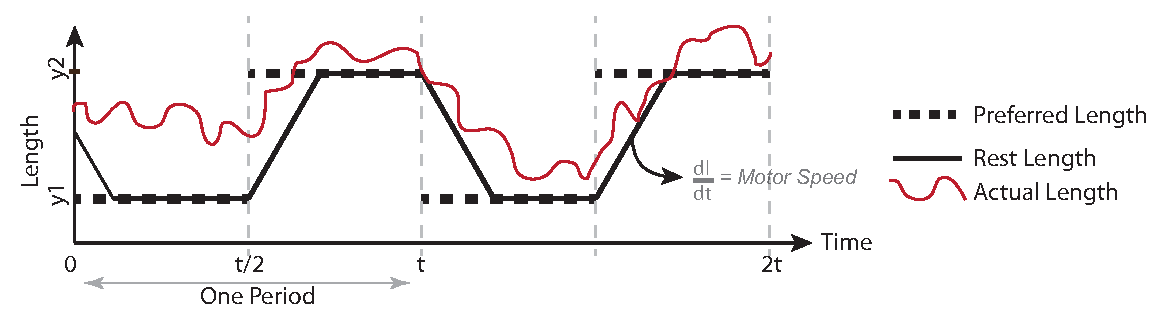
\includegraphics[width=\columnwidth]{tex/ASME-journal/fig/signal.eps}
\caption{An example signal with 2 sub-intervals with preferred lengths of y1 and y2 and periodicity t.}
\label{fig:signal}
\end{figure}

When the function is expanded to \(n = k\) it takes the form of

\begin{align}
F(t') =
  \begin{cases}
    y1       & \quad \text{for} t' \in [0, t_{1}]\\
    y2       & \quad \text{for} t' \in (t_{1}, t_{2}]\\
    \vdots   & \quad \vdots \\
    yk       & \quad \text{for} t' \in (t_{k-1}, t]\\
  \end{cases}
\end{align}

and it can easily be shown that as \(n \to \infty\) any arbitrary signal may be generated.
To generate a signal, the only parameters needed are number of sub-intervals and rest length values for each sub interval. 
For the specific example given in Figure \ref{fig:signal}, the number of subintervals is 2 and y1 and y2 are the values of preferred rest lengths for those intervals. 

% Let's assume that the periodicity of the signal is $t$ and WE represent the signal as $F(x)$ , $x$ being time within interval $[0,t]$. There are many possible ways to represent this control function. For instance a natural choice would be a sine wave, or a series of overlapping waves to form more complex control policies. To reduce complexity, in this paper WE use an even simpler control model: WE break down each control interval into sub-intervals and assign different preferred rest lengths for each sub-interval.  Considering the limited velocity of the motors, the motor will slowly move to reach these selected points during those sub-intervals. The control model is essentially a set of overlapping square waves. As an example, WE can divide one period to 2 sub-intervals, where the motor will have a preferred length of $y1$ for the first half of the signal, and $y2$ for the second half of the signal. With the motor moving towards $y1$ and $y2$, the resulting signal will be similar to the Figure \ref{fig:signal}. 


% To generate a signal, the only parameters needed are number of sub-intervals and rest length values for each sub interval. 
% For the specific example given in Figure \ref{fig:signal}, the number of subintervals is 2 and y1 and y2 are the values of preferred rest lengths for those intervals. 
% The example given in the Figure \ref{fig:signal} is a simple signal, and while number of sub-intervals is low, the complexity of the signals that can be generated is limited. 
% On the other hand, the complexity of the possible signals increases with the number of sub-intervals. 
% Due to this, from now on, WE will refer to this parameter as the complexity degree  ($n$) of the signal. 
% Depending on the complexity degree and the values of $y_1,y_2,...y_n$, the shape of the signal can change between typical trapezoid, zigzags, stairs or combination of those. 

% To summarize, the complexity of the signal depends on $n$ and each controller has $n$ number of inputs depending on the complexity selected. The rest lengths of the signal follows this signal, and actual lengths of the MUSCLES change according to other MUSCLES and interaction of the robot with the environment. Each controller has a separate signal and it controls only one of the motors. 24 motors controls 24 MUSCLES independently but affecting each other with the common goal of rolling locomotion.


% While the control parameters  to generate the signal are straightforward, the interaction between these signals to reach a rolling behavior is highly complex. As explained before, the  nonlinear and oscilattory nature of the problem makes the tensegrity hard to control with classical control methods. The consequences of specific signal combinations can be simulated, but finding the correct signal parameters for a specific behavior is not possible. In this section WE explore how WE can use the simulation combined with a fitness evaluation to implement an evolutionary algorithm that can evolve a set of control parameters that leads to the desired behavior.

% Evolutionary algorithms are a family of biologically inspired learning methods, where new candidate solutions for a problem are generated, evaluated and eliminated repeatedly \cite{back1997handbook}. Evolutionary algorithms consists of the cycle of  forming new members, assigning fitness and selecting the most fit members. This cycle is called a generation and it is repeated until desired behavior is obtained. 

\subsubsection{Algorithm and Learning Method}
The problem is episodic, the agents have 60 seconds to test their policies. At the end of each episode these candidates are evaluated according to their performance. 
Performance is then measured as the distance covered in 60 seconds. 
Formally, the evaluation is defined as

\begin{equation}
\label{eq:r}
f = d(y_{0,0},y_{0,1},...,y_{0,n},y_{1,0},...,y_{24,n}) \;,
\end{equation}

where, $y_{i,j}$ is the rest length for the $i$th controller and $j$th subinterval. 
Depending on the complexity of the signals ($n$) selected, there are $24 * n$ parameters to learn. 
% For this study, WE used the historical average method that WE previously developed and tested with earlier versions of NTRT to obtain rolling behavior using sine wave signals (REF). 
In order to learn these parameters, this method uses a historical average co-evolutionary algorithm.
In historical average, each member receives its fitness according to the average of their performances.
If a member survives for the next generation (is not eliminated or mutated) the member keeps  its previous experiences. 
At each generation, the fitness assignment is the average of this growing history of past evaluations. 
% The overall cooperative coevolutionary algorithm with historical average fitness assignment can be found in Algorithm \ref{Alg:CCEA-AA}.
The algorithm used can be found in Algorithm~\ref{Alg:CCEA-AA}.

% Note that the decomposition of the distance function $d$ is not readily obtainable in closed form. Instead it must be computed from observing simulations or measured from a physical implementation. Also note that OUR evaluation does not explicitly take any behavior into account besides the distance moved (final position - initial position). Tensegrities can exhibit many different gaits, ranging from hopping to rolling, and many different paths, ranging from spirals to straight lines. However, tensegrities that maximize final vs initial position tend to roll towards one direction. Deviations from this pattern tend to hurt performance.


\begin{algorithm}[th]
 \SetAlgoLined
 \KwData{Population of $n$ elements for each agent}
 \For{i=1..$k$}{
  $random team \leftarrow \emptyset$ \;
  \ForAll{Populations} 
  {
  	$random_team \leftarrow random_agent$\;
  }
  score = evaluate($random_team$) \;
  \ForAll { agents $\in$ $random_team$}
  {
  	agent.history $\leftarrow$ score \;
%  	\If{score $>$ agent.score}
%  	{
%  		agent.score $=$ score \;
%  	}
  }
  }
 \ForAll{ Populations }
 {
   \ForAll { agents}
   {
   	   agent.fitness = average(agent.history) \;
   }
 	order population according to the fitness\;
 	eliminate the last $z$ members\;
 	copy the first $z$ to the last $z$\;
 	mutate the last $z$\;
 	clear history for the last $z$\;
 }
 
\caption{Cooperative coevolutionary Algorithm with Historical Average}
\label{Alg:CCEA-AA}
\end{algorithm}

% The problem that WE are working on is distributed by nature. The controllers are independent and there is not a centralized mechanism. To work on such problems, cooperative coevolutionary algorithms (CCEA) is a class of algorithms that extends evolutionary algorithms. Instead of one particular solution for the problem, there are multiple agents. Multiple agents have to coordinate to solve a problem or to optimize an outcome \cite{wiegand2003analysis}. Each agent has a separate population that evolves independently. On the other hand, to evaluate the members of these separate populations, the agents have to form a team for fitness assignment, because the task needs cooperation of the agents to maximize the rolling behavior. At each experiment 1 member from each population are chosen randomly to form a team. This set of policies form the team for that experiment. In OUR problem, WE have 24 agents which means 24 populations.

% Each agent optimizes $n$ parameters while they are judged based on their performances within different teams formed during evaluation phase. At each evaluation phase, each member is evaluated multiple times. To move on to the elimination phase, each member has to be assigned a single fitness number using these values. The literature contains multiple approaches to this problem such as taking the maximum score (leniency), testing each member with best team so far (hall of fame) or average score \cite{wiegand2003analysis,panait2008theoretical,Iscen:2013aa}.

% For this study, WE used the historical average method that WE previously developed and tested with earlier versions of NTRT to obtain rolling behavior using sine wave signals (REF). In historical average, each member receives its fitness according to the average of their performances, moreover, if a member survives for the next generation (is not eliminated or mutated) the member keeps  its previous experiences. At each generation, the fitness assignment is the average of this growing history of past evaluations. The overall cooperative coevolutionary algorithm with historical average fitness assignment can be found in Algorithm \ref{Alg:CCEA-AA}.


\subsubsection{Learning Results}
An example learning session is shown using signals with complexity ($n$) of 5 and period ($t$) of 4 seconds.  
Figure \ref{fig:learning} illustrates the distance rolled by the robots over the course of learning. 
Starting with 0 meters, the robots converge to rolling over 32 meters in 60 seconds. 
This result shows that successful learning of rolling locomotion using CCEA is possible. 
% In Section \ref{sec:platform} WE discussed when a policy is labeled as unfeasible during learning.  
The second line at the same Figure (Figure \ref{fig:learning}) shows the rate of unfeasible policies that are tried while learning to roll. 
While converging to rolling locomotion, unfeasible policies drop to 0. 
This shows that the learned policy lies within simulated parameters set by the user.

\begin{figure}[t]
\centering
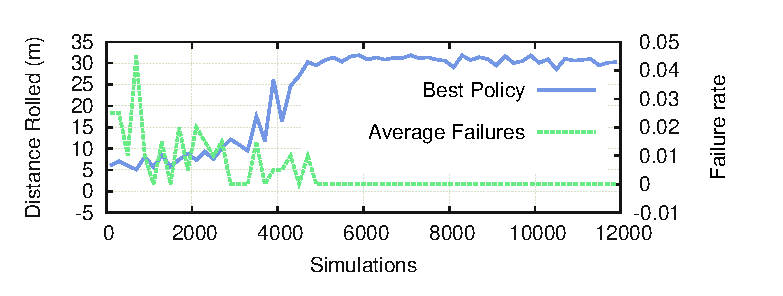
\includegraphics[width=\columnwidth]{tex/ASME-journal/results/failures/learningVsFailures.eps}
\caption{The performance of the robots during the learning session for signals of complexity 5 and period of 4 seconds. As a side result, the percentage of the policies that were failed to stay in reasonable limits are shown with the second line. }
\label{fig:learning}
\end{figure}

% Considering that the robot has a shape that is similar to a sphere with a diameter of 1.5 meters, rolling 32 meters  means  approximately 7 revolutions in a minute. 
% This results in 8 seconds per revolution. 
% Considering that WE selected 4 seconds as periodicity of the signal, the learned signals  provide half revolution, and applying same signals also results in the other half of the one complete revolution.  
% This supports the reasoning behind selecting periodic signals to obtain rolling locomotion as a periodic movement of the robot.

% \begin{figure}[t]
% \centering
% 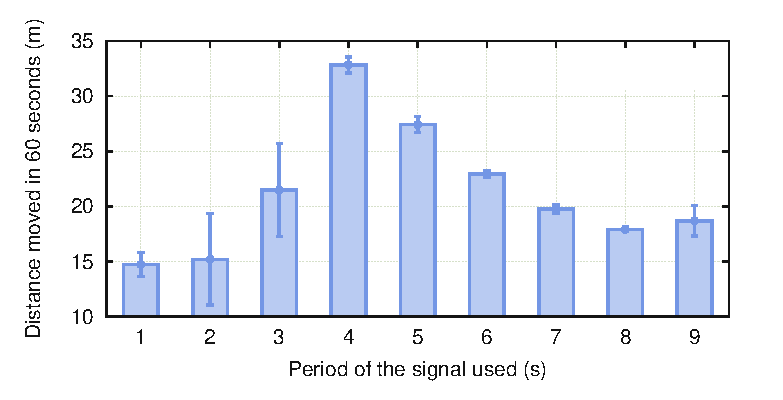
\includegraphics[width=\columnwidth]{tex/ASME-journal/results/period/period.eps}
% \caption{The performance of the converged policies after learning for signals with periods of different lengths, while the complexity is fixed to 5 points. The best performance is reached with signals that are repeated every 4 seconds. Signals with longer periods have a decreasing performance proportional to the inverse of the periodicity.}
% \label{fig:period}
% \end{figure}


% \begin{figure}[t]
% \centering
% 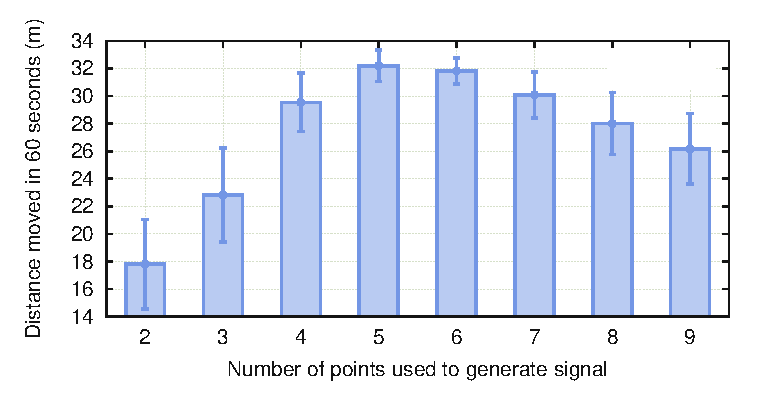
\includegraphics[width=\columnwidth]{tex/ASME-journal/results/complexity/complexity.eps}
% \caption{The performance of the converged policies after learning for signals with different complexity levels, while the periodicity is fixed to 4 seconds. The best performance is reached with signals that use 5 points. Less complex signals cannot generate rolling locomotion, and more complex signals are hard to learn.}
% \label{fig:complexity}
% \end{figure}

% % The first set of experiments illustrated when $n$ and $t$ are selected as 5 and 4 (4 seconds with complexity of 5). Next, WE investigate the results of learning using signals with different complexity and periodicity. Figure \ref{fig:period} shows the converged behaviors when WE fix  $n$ to 5 and learn using variable $t$. Note that the signal used for different values of $t$ is not the same. The signals are learned from scratch for each value of $t$. 

% % Clearly, the peak is when the signals have periods of 4 seconds (frequency of 0.25 Hz). When WE shorten the period below 4 seconds, the robot cannot learn to roll. One can think that providing the same signal with a higher frequency can provide the same rolling behavior, but when the tensegrity deforms to start rolling with a higher speed, the contact forces from the ground and the reaction of the structure changes completely. When WE increase the periodicity to longer than 4 seconds, the frequency drops and the performance gradually decreases as expected. Moreover,  the rolled distance is linearly proportional to the frequency. For the values of $4$ to $8$ seconds, the performance divided by the frequency give the same value ($\frac{33}{1/4} \simeq \frac{27}{1/5} \simeq \frac{22.5}{1/6} \simeq \frac{19}{1/7} \simeq 132 $). 


% Next, WE investigate the effects of different signal complexity level to the learning.  The period is fixed at 4 seconds, because it gave the best score combined with the complexity of 5 in previous set of experiments (Figure \ref{fig:period}). WE started with the complexity of 2, where the signal is simplest possible. It alters between one high value for the first 2 seconds, and one low value for the last 2 seconds. WE increase the complexity up to 9 points. The result is illustrated at Figure \ref{fig:complexity}.  The first conclusion is that signals with complexity 2 cannot succeed at learning to roll, but the performance increases with higher complexity. Clearly the controllers need more complex signals to provide rolling locomotion. The peak performance is reached at complexity 5, where the preferred length alters between 5 different points during 5 intervals of 0.8 seconds each. 

% The second conclusion of this experiment is seen when the complexity increases even further.  The learned behavior gradually decreases and error bars show that statistical significance goes down. The reason behind this behavior is that the parameters to learn increase linearly, and the problem to learn becomes linearly harder for each controller. Since all the controllers learn simultaneously while interacting with each other, overall hardness of the problem is increased even further. The error bars show that in more complex problems, some statistical tests reach good results while some of them fail completely due to the hardness of the problem.

% \subsection{Analyzing the Rolling Behavior}
% \label{sec:openResults}

% In previous section, WE showed that learning to roll for a tensegrity robot succeeds with signals of right periodicity and complexity. In this section, WE look at the learned behavior and analyze 
% the feasibility of the behavior, lengths and tensions during rolling, converged signals and robustness of the behavior.

% As a sample learning behavior, WE select one of the learned behaviors with periods of 4 seconds and complexity of 5. The learning process for this behavior was illustrated in Section \ref{sec:learning} and Figure \ref{fig:learning}. For each simulation, the robot tests different policies for 60 seconds, and the distance moved is marked as the score. The policies that are tested are updated according to the Cooperative Coevolutionary Algorithm with Historical Average (Algorithm \ref{Alg:CCEA-AA}). For this particular experiment, the robots reach the performance of rolling 32 meters around 5000 simulation steps. As a side result, the percentage of failed policies (due to high tension) reaches 0.

% \begin{figure}[t]
% \centering
% 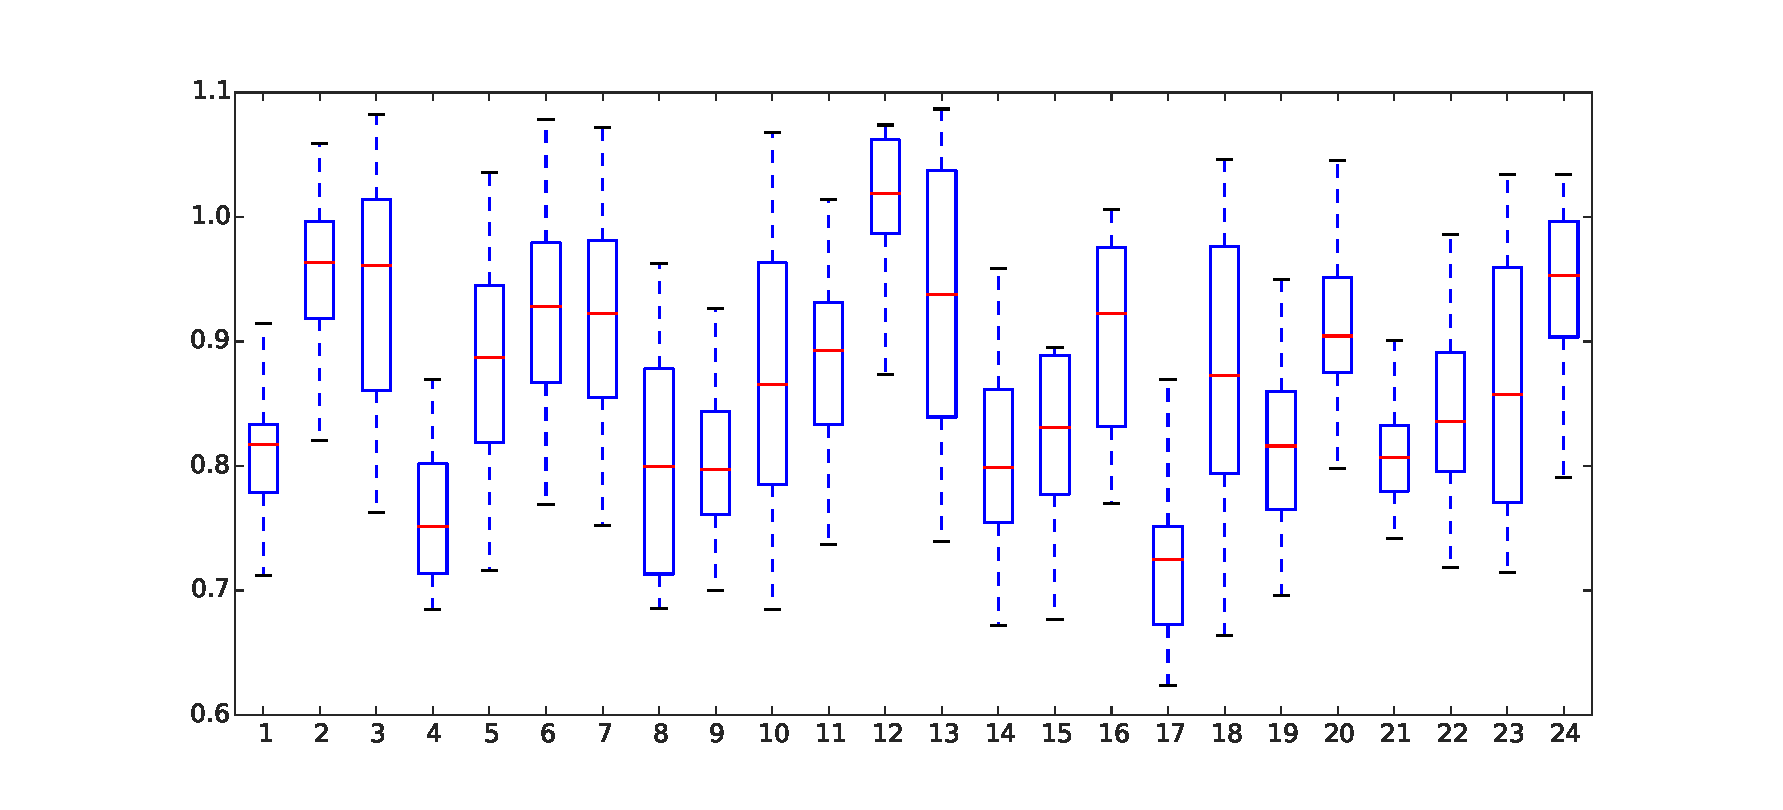
\includegraphics[width=\columnwidth]{tex/ASME-journal/results/signals/policy.eps}
% \caption{A sample learned policy for 24 motors is illustrated. For each signal, the red line at the center shows the mean of the signal and the box and the dashed lines show the interval that the signal lies in.}
% \label{fig:policy}
% \end{figure}

% First, WE take this learned behavior and look at the learned policy. Figure \ref{fig:policy} shows the intervals that each muscle's length lies within.  The muscles' lengths vary from 0.7 m to 1.1 m. While some of the MUSCLES such as 1 and 21 have minimal change in length, some of them (such as 13 and 23) changes bigger intervals. Another remark is that, the mean of the signal (that is noted by the red horizontal line) is not necessarily at the center of the interval that the signal lies in. This is one difference that more complex signals provide. For example, the length of the muscle number 1 is mostly around 0.82 m, but it reaches as low as 0.7 once in a while.
 
% \begin{figure}[th]
%         \centering
%         \begin{subfigure}[b]{0.9\columnwidth}
%                 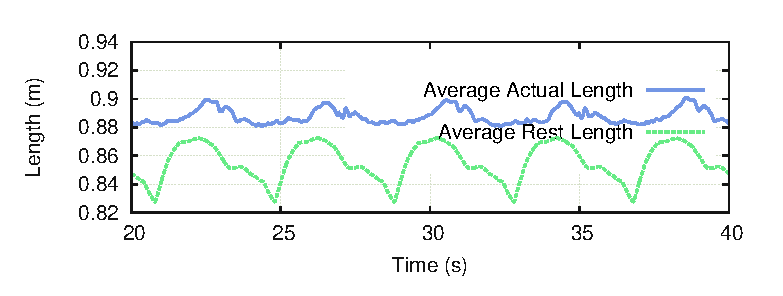
\includegraphics[width=\textwidth]{tex/ASME-journal/results/tension-energy/lengths.eps}
%                 \caption{Average Rest Lengths and Actual Lengths of The Muscles}
% 				\label{fig:lengths}
%         \end{subfigure}\\
%         \begin{subfigure}[b]{0.9\columnwidth}
% 				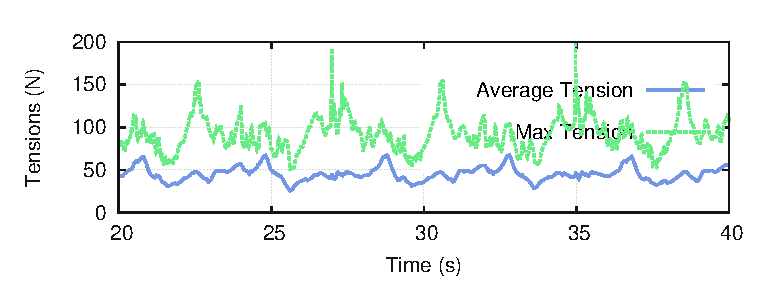
\includegraphics[width=\textwidth]{tex/ASME-journal/results/tension-energy/tensions.eps}
%                 \caption{Average and Maximum Tensions of the Muscles}
% 				\label{fig:tensions}
%         \end{subfigure}\\
%         \begin{subfigure}[b]{0.9\columnwidth}
%                 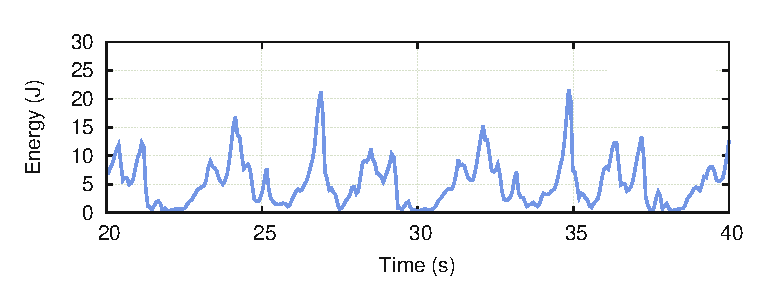
\includegraphics[width=\textwidth]{tex/ASME-journal/results/tension-energy/tensKinEnergy.eps}
%                 \caption{Kinetic Energy of the Tensegrity Robot}
%                 \label{fig:KinEnergy}
%         \end{subfigure}\\
%          \begin{subfigure}[b]{0.9\columnwidth}
%          		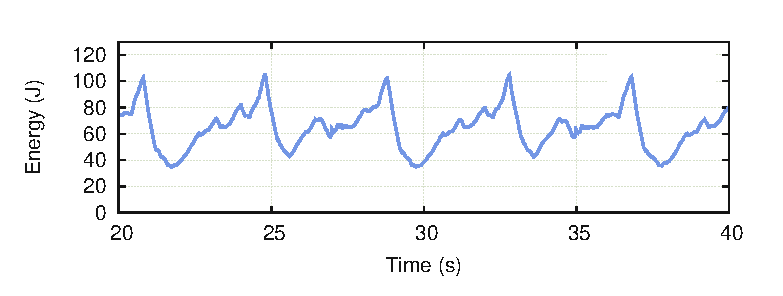
\includegraphics[width=\textwidth]{tex/ASME-journal/results/tension-energy/tensPotEnergy.eps}
%                 \caption{Total Potential Energy Stored in Muscles}
%                 \label{fig:PotEnergy}
%         \end{subfigure}
%         \begin{subfigure}[b]{0.9\columnwidth}
%          		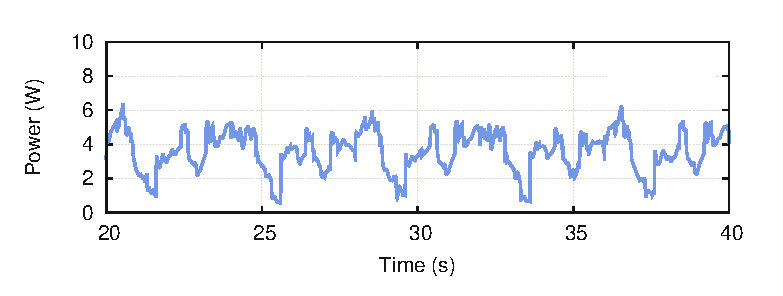
\includegraphics[width=\textwidth]{tex/ASME-journal/results/tension-energy/power.eps}
%                 \caption{Power Used by the Motors to Roll}
%                 \label{fig:power}
%         \end{subfigure}
%         \caption{Illustration of different aspects of the Tensegrity Robot over time, during rolling locomotion. The used signals for MUSCLES repeat themselves every 4 seconds. The tensegrity robot completes one revolution in 8 seconds. Tensions, Lengths and Power usage of the robot stays in OUR defined limits for the hardware. }
%         \label{fig:RollingAnalyze}
% \end{figure}


% One way to analyze rolling behavior is looking at the average lengths and tensions of the MUSCLES in addition to the potential and kinetic energy of the structure. First, WE look at how the actual lengths of the MUSCLES change compared to the signals provided. Figure \ref{fig:lengths} shows the average rest length of the MUSCLES (signal provided) and the average actual length of the muscles. The area between the two lines shows the stretch of the MUSCLES due to the tension. The most interesting fact about this graph is the difference of frequencies for the two lines. Although the signals that are provided to the MUSCLES repeat themselves every 4 seconds, the actual lengths repeat themselves every 8 seconds. This supports OUR previous conclusion about using signals that have periodicity of 4 seconds can conclude in revolutions that take 8 seconds. The first half of the roll and second half of the roll use same signal, but the ground interactions make the actual lengths differ.



% During the rolling, the average and maximum tensions of the MUSCLES are illustrated in Figure \ref{fig:tensions}. The average tension is low, stays around 60 N. The second line shows the 
% the tension of the muscle with longest stretch at each particular time of the simulation. The value goes up to 200N staying in values that OUR hardware design can handle. The maximum tension graph also repeats itself every 8 seconds as expected.

% When WE observed  the gait learned using OUR simulator, WE see the rolling locomotion does not have a constant speed. Instead, it slows down and speeds up periodically during each revolution. To illustrate this behavior, WE look at the total kinetic energy of all the rods over time in Figure \ref{fig:KinEnergy}. If WE take the interval between two peak points (when t=27 and t=35), the kinetic energy stays at zero for 1 second around t=30s. Moreover, the repetitive acceleration and deceleration can be clearly seen. This behavior creates an inefficiency in terms of energy for the gait. There are two main reasons for this behavior: First, the learning algorithm only optimizes the distance rolled, not the energy spent during motion. Optimizing more than one criteria  is actually part of OUR future work. Second, in this work, WE are testing open loop controllers. Using some feedback from the robot (such as lengths, tensions or orientation) having a smoother rolling experience can be possible. This is also another future work that WE explain in Section \ref{sec:conclusion}.

% Next, WE observe the potential energy stored in the muscles. Figure \ref{fig:PotEnergy} shows the pattern that repeats itself every 8 seconds as expected. First 4 seconds and second 4 seconds are similar but they slightly differ due to different environment reaction during the second half of a complete roll. The pattern shows an overall behavior of increasing the potential energy slowly over time, and releasing it. This matches the kinetic energy behavior that WE observed in Figure \ref{fig:KinEnergy}. The kinetic energy of the structure increases during the few seconds following the moment potential energy is released (i.e. t=25s).

% The last set of experiments analyzes the approximated power usage by the motors during the rolling locomotion. In simulation, the power consumption is approximated using the current tension of the element  and the constant speed that the motors shortens the muscles. As WE explained earlier, the learned behavior is not optimized to be power efficient for this study. On the other hand, WE want to make sure that it is within limits of motors and batteries that will be used in the hardware. Figure \ref{fig:power} illustrates the average power consumption of the MUSCLES that varies between 2 to 6 W per muscle. Considering that the motors always pull against the tension (and all the MUSCLES are  tight all the time) this value is considerably low. Moreover, it is always possible to lower this value by using a feedback controller in future work.


% \section{Analyzing the Roles of Different Muscles}
% \label{sec:signals}



% \begin{figure}
%         \centering
%         \begin{subfigure}[b]{\columnwidth}
%         		\centering
%                 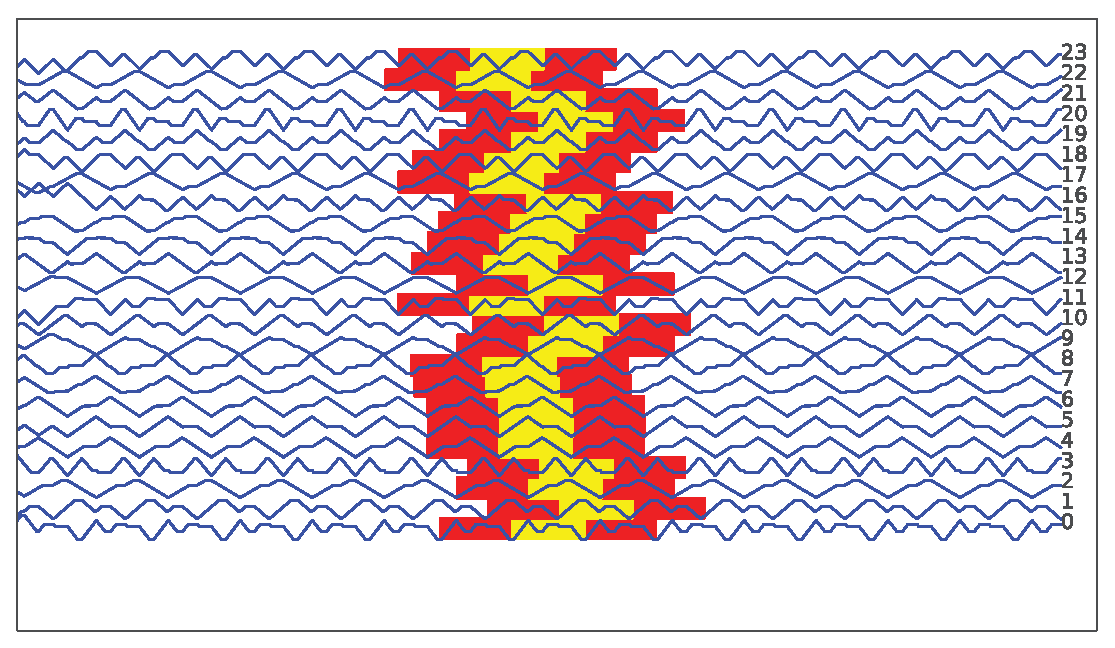
\includegraphics[width=0.7\textwidth]{tex/ASME-journal/results/signals/aligned1.eps}
%                 \caption{The signals of the 24 MUSCLES normalized between [$i$,$i$+1] for muscle $i$. After correlation using time offsets, the highest correlated intervals of 4 seconds are  marked with red,yellow,red pattern. }
% 				\label{fig:aligned1}
%         \end{subfigure}\\
%          \begin{subfigure}[b]{\columnwidth}
%         		\centering
%                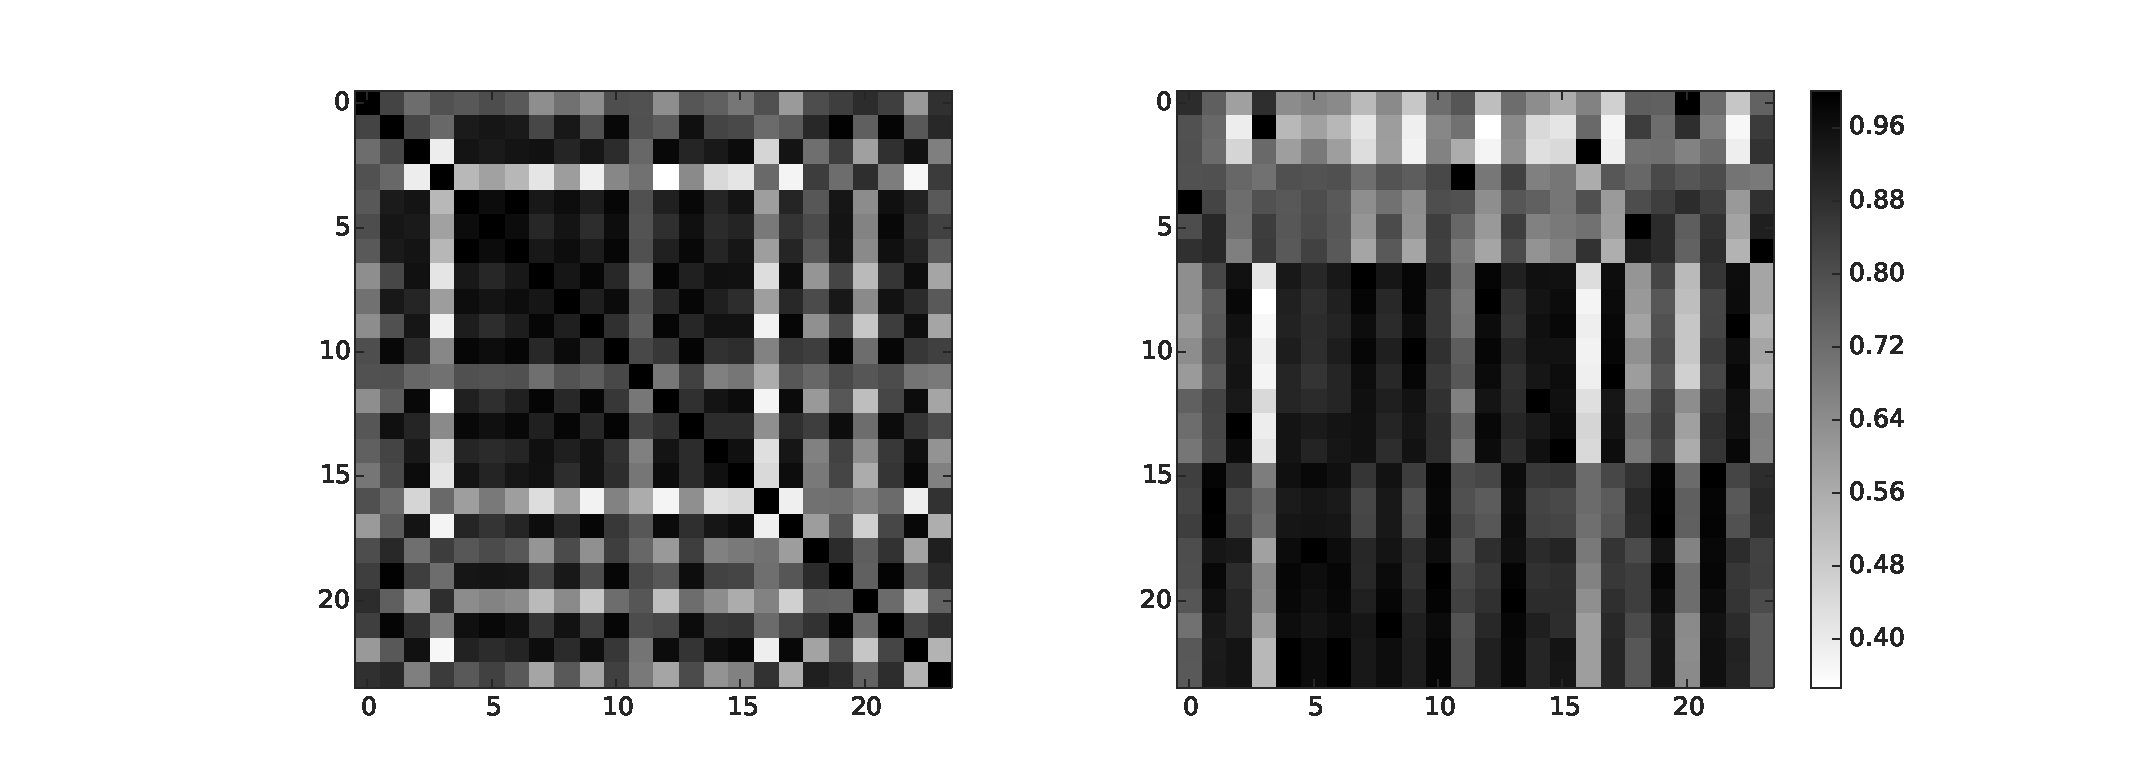
\includegraphics[width=0.7\textwidth]{tex/ASME-journal/results/signals/correlation.eps}
%                 \caption{24x24 Correlation matrix of signals used for each muscle before and after reordering using hierarchical clustering. }
% 				\label{fig:correlation}
%         \end{subfigure}\\
%         \begin{subfigure}[b]{\columnwidth}
%         		\centering
%                 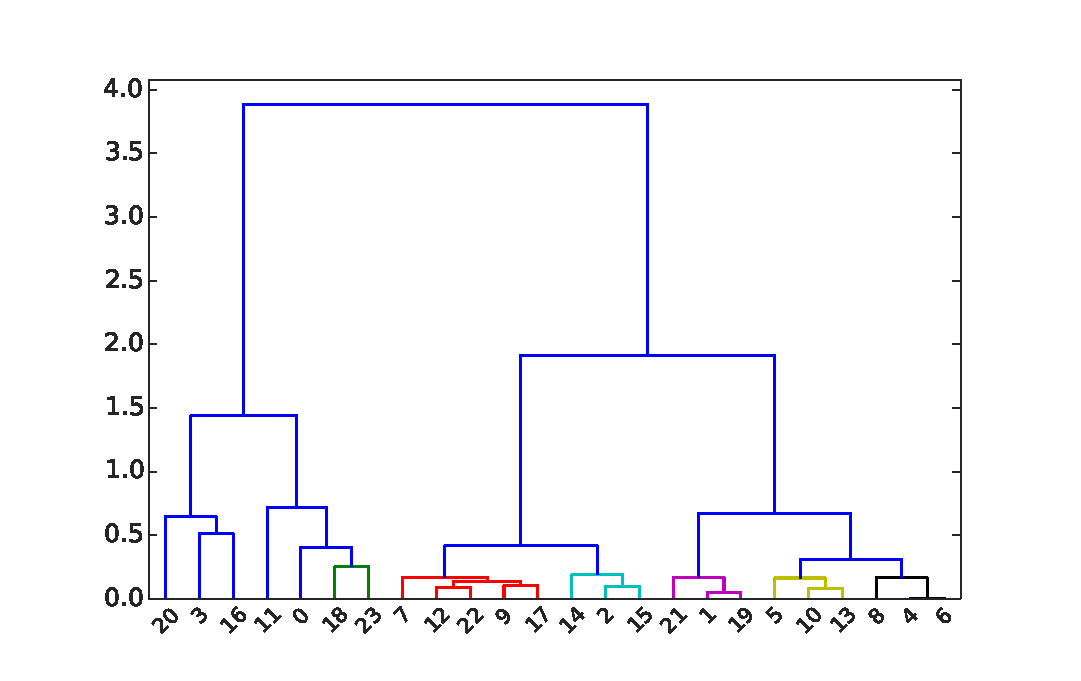
\includegraphics[width=0.7\textwidth]{tex/ASME-journal/results/signals/clustering.eps}
%                 \caption{Result of Hierarchical clustering to cluster and reorder similar signals}
% 				\label{fig:clustering}
%         \end{subfigure}\\
%         \begin{subfigure}[b]{\columnwidth}
%         		\centering
%                 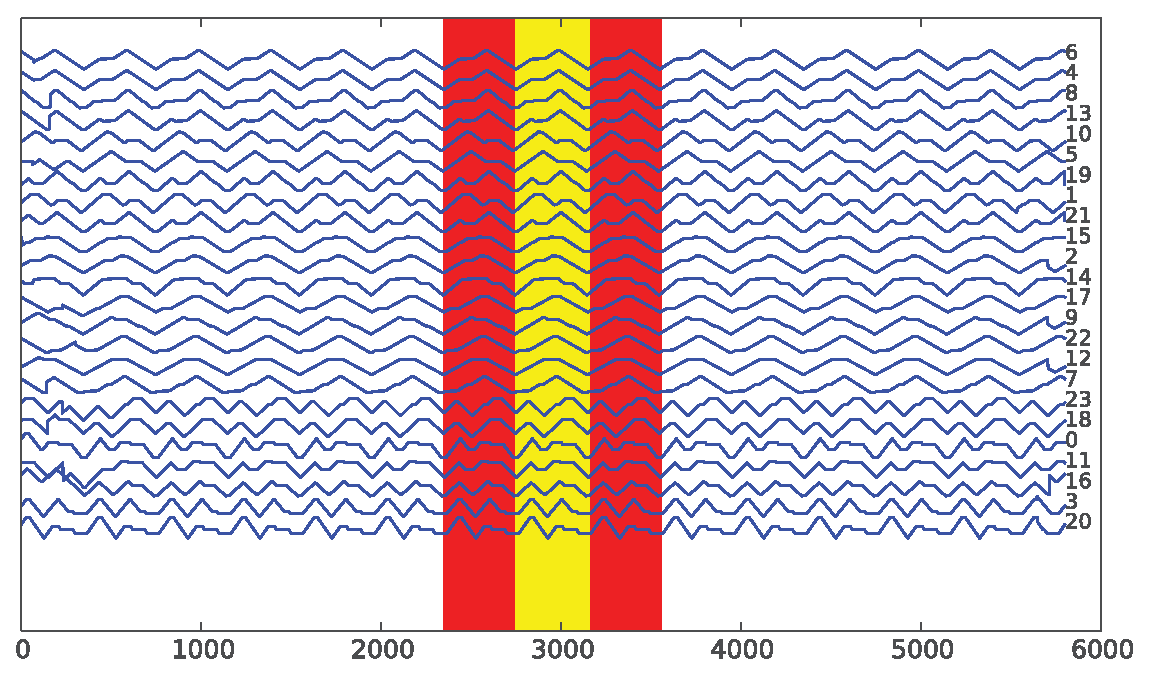
\includegraphics[width=0.7\textwidth]{tex/ASME-journal/results/signals/aligned2.eps}
%                 \caption{The signals for the MUSCLES when they are shifted according to the highest correlation and reordered according to the hierarchical clustering. }
% 				\label{fig:aligned2}
%         \end{subfigure}
%         \caption{The process of analyzing the signals used for the muscles. The signals are shifted and reordered to show similarities. Subfigure (d) shows that groups of signals have similar patterns.}
%         \label{fig:correlationAll}
% \end{figure}

% Next, WE analyze the signals further by looking at their shapes and correlation between them. The top half of the Figure \ref{fig:aligned1} shows all 24 signals when they are normalized between 0 and 1. The purpose of this experiment is to show similarities of signals and different types of signals learned at the end of coevolution. First, WE look at the correlation between signals. For each signal, red-yellow-red area highlights the interval that maximizes correlation with other signals. At this ordering, it is hard to see similarities between signals. In Figure \ref{fig:aligned2}, WE shift the signals so that their selected intervals match, then WE use hierarchical clustering (Figure \ref{fig:clustering}) to group the signals according to the similarity metric. 

% After reordering the signals, Figure \ref{fig:aligned2} shows that half of the signals have one peak high and one low, but the other half have 2 signals that are more complex with 2 peak points. This result gives us multiple conclusions. First, the learning algorithm makes use of the complexity provided. Although a subset of the signals is simple, but another subset has more complex signals with  multiple peak points that can only be generated with complexity coefficients that are higher than 3. The subsets of the signals that are similar can be regenerated using different parameters but the same formula. Let's consider a normalized signal as $f(x)$. The formula $g(x)=A+B*f(x+C)$ can produce similar signals for different values of $A$, $B$ and $C$. Using this idea, all 24 signals can be reproduced using 3 to 4 base functions and different parameters. This gives us a hint about why many papers in literature proposes to use central pattern generators to control tensegrity robots. 

% The last set of results show how critical each muscle is for a given rolling locomotion. WE take the tensegrity robot with the learned policy and disable one of the MUSCLES and observe the effect of such a failure on overall behavior. Figure \ref{fig:disable1} shows that performance depends on which muscle fails. For a significant number of muscles, using the same algorithm still provides rolling behavior with similar performance.  On the other hand some MUSCLES play a critical role for that specific policy.

% \begin{figure}[t]
% \centering
% 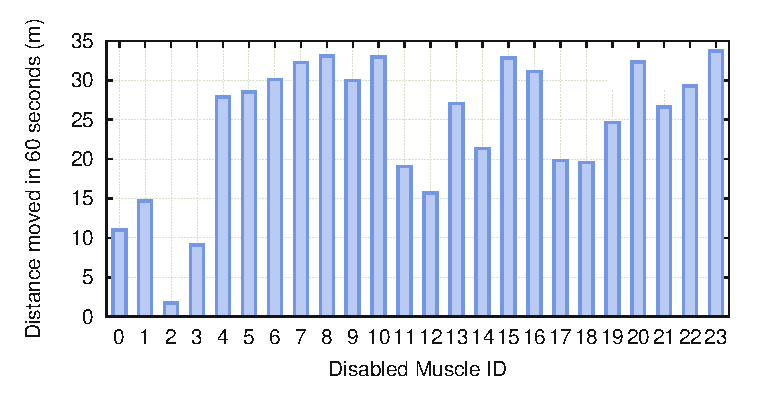
\includegraphics[width=\columnwidth]{tex/ASME-journal/results/testing-disabling1/disabled.eps}
% \caption{The performance of the learned policy, when WE disable one of the muscles. Learned policy is partially robust to failures of some of the muscles. }
% \label{fig:disable1}
% \end{figure}


\subsection{Mirror Descent Guided Policy Search}
\label{sec:mdgps}

%Policy search algorithms aim to find a good policy by directly searching through
%the space of policy parameters. 
Guided Policy Search utilizes supervised policy learning to leverage a series of non-generalized optimized local polices to learning a generalizable global policy~\cite{lk-gps-13}.
These non-generalized optimized local policies, $\trajdist_i(\at|\st)$, only successfully work from specific initial states and require full state information.
Guided Policy Search allows for the use of simple and efficient methods for training the local policies,
such as trajectory optimization methods when there is a known model, or
trajectory-centric reinforcement learning methods~\cite{la-lnnpg-14}.

In this work, a modified version of Guided Policy Search is used based on mirror descent~\cite{ml-gpsam-16}, called Mirror Descent Guided Policy Search (MDGPS).
This version optimizes the global policy by sampling the current iteration's local polices and approximates the minimum divergence between the global policy and the local policies.
To optimize the local polices, $\return(\params)$ is minimized such that there is a bound on the Kullback–Leibler divergence (KL-divergence) between the local policy and the linearized global policy $\bar\policy_{\params{i}}$~\cite{bagnell2003covariant,ps-rlmsp-08,pma-reps-10,slmja-trpo-15}.
For clarification, the KL-divergence is a measure of how much information is lost when using a probability distribution to approximate another distribution.
A generic MDGPS algorithm is shown in Algorithm~\ref{alg:mdgps}.

Policy learning machine learning algorithms, commonly called policy search algorithms, are used to directly search the policy parameter space and are alternatives to value function based reinforcement learning algorithms~\cite{bagnell2003policy}. 
%Formally, we wish to find a setting of the
This algorithm tries to find a set of
policy parameters $\params$ which optimizes the policy
$\policy_{\params}(\at|\obs_t)$ with respect to the expected cost. 
%In the finite-horizon episodic setting,
With a finite set of episodes, 
the expected cost under the policy is given by
$\return(\params)=\sum_{t=1}^{T}\mathbb{E}_{\policy_{\params}}[\cost(\st,\at)]$,
where $\cost(\st,\at)$ is the cost function. 
%Here $\st$ denotes the state of our
$\st$ is the state of the
system at time $t$, $\obs_t$ is the observation of the state at time $t$,
and $\at$ is the action at time $t$.

%Guided policy search algorithms use supervised learning to train the policy,
%with supervision coming from several local policies $\trajdist_i(\at|\st)$ that
%are optimized to succeed only from a specific initial state of the task using
%full state information. 
% This is much simpler than the goal of the global
% policy, which is to succeed under partial observability from any initial
% condition sampled from the initial state distribution. These simplifications
% allow the use of simple and efficient methods for training the local policies,
% such as trajectory optimization methods when there is a known model, or
% trajectory-centric reinforcement learning methods~\cite{la-lnnpg-14}. 

% In this work, the 
% The specific algorithm used in this work is MDGPS, which interprets GPS as
% approximate mirror descent on $\return(\params)$~\cite{ml-gpsam-16}. The local
% policies are optimized to minimize $\return(\params)$ subject to a bound on the
% KL-divergence between the local policy $\trajdist_i$ and the linearization of
% the global policy $\bar\policy_{\params{i}}$, following previous
% work~\cite{bagnell2003covariant,ps-rlmsp-08,pma-reps-10,slmja-trpo-15}.
% Optimizing the global policy is done using the samples collected in the current
% iteration, which are used in a supervised fashion to approximately minimize the
% divergence between the global policy and the local policies.

\setlength{\textfloatsep}{12pt}
\begin{algorithm}[tb]
    \caption{Mirror descent guided policy search (MDGPS)}
    \label{alg:mdgps}
    \begin{algorithmic}[1]
        \FOR{iteration $k = 1$ to $K$}
            \STATE Run either each $\trajdist_i$ or $\policy_{\params}$ to
            generate samples $\{\traj\}$
            \STATE Set
            $\trajdist_i\leftarrow\argmin_{\hat\trajdist_i}\mathbb{E}_{\hat\trajdist_i}[\cost(\traj)]~s.t.~D_{KL}(\hat\trajdist_i\|\bar\policy_{\params{i}})\leq\epsilon$
            \STATE Train $\policy_{\params}$ using supervised learning on
            $\{\traj\}$
        \ENDFOR
    \end{algorithmic}
\end{algorithm}

% The generic MDGPS algorithm is summarized in Algorithm~\ref{alg:mdgps}. On line
% 2, samples are collected by running either the global policy or the local
% policies. This choice between ``on-policy'' and ``off-policy'' sampling is
% detailed in previous work~\cite{ml-gpsam-16}. On line 3, the algorithm improves
% the local policies using an LQR-based update using fitted local linear models:
% the samples are first used to fit time-varying linear dynamics for each local
% policy, and these fitted dynamics are then used with a KL-constrained LQR
% optimization to update the linear-Gaussian local policies. This corresponds to a
% simple model-based trajectory-centric reinforcement learning method, and further
% details can be found in prior work~\cite{la-lnnpg-14}. On line 4, the global
% policy $\policy_\params(\at|\st)$ is updated using supervised learning, with the
% training data corresponding to the states along the samples, with actions given
% by the new updated local policies. This causes the global policy to ``catch up''
% to the newly improved local policies, improving its behavior for the next
% iteration.


\subsubsection{Optimizing Periodic Gaits with MDGPS}
\label{sec:chains}

Using the MDGPS method stated in section~\ref{sec:mdgps}, a periodic rolling gait for \SB{} was learned using single transitions between faces mentioned in section~\ref{basic_locomotion} as the local policies and how to transition between them using limited sensor data as the global policy. 
In order to obtain this stable periodic rolling gait, the task is split across several policies, each optimized over a small time segment.
After establishing a desired behavior across the states seen by the policies, a global policy is learned that can generalized the behavior of the local polices based on the Guided Policy Search framework.

% The efficiency and speed of model-based policy optimization methods, such as the
% LQR-based method used to optimize the local policies in MDGPS, is due in large
% part to the fact that dynamic programming can allow for large changes to a
% policy that would be impractical with purely sample-based model-free
% methods~\cite{la-lnnpg-14}. However, in complex stochastic domains, such as the
% contact-rich dynamical system of a rolling tensegrity robot, the accumulation of
% uncertainty and variability under an unstable policy can make it difficult to
% apply dynamic programming over the long horizons needed to establish a periodic
% gait. We demonstrate this effect through our experimental results in
% Section~\ref{sec:simresults}. 
% In this section, we describe how we can obtain a
% policy with stable periodic behavior by first splitting the task across multiple
% policies, each optimized over a smaller time segment where it is easier to apply
% dynamic programming, and establishing good behavior across the range of states
% visited by these policies. Following the framework of GPS algorithms, we
% subsequently learn a global policy that can generalize the behavior of the local
% policies and encapsulate a successful periodic gait into a single policy.

GPS algorithms such as MDGPS use supervised learning to learn a global policy,
where the supervision comes from several local policies $\trajdist_i(\at|\st)$,
$i\in\{1,\ldots,C\}$. Each local policy is trained from a different initial
state, where $C$ is the chosen number of initial states. Each local policy is
optimized over $T^{\trajdist}$ time steps, and we wish to learn a global policy
$\policy_{\params}(\at|\obs_t)$ that can succeed by generalizing the behavior of
these local policies over an episode of length $T^{\policy}$.

In locomotion
tasks, we ideally want the global policy to exhibit continuous successful
behavior, i.e., $T^{\policy}=\infty$, and we can empirically determine
$T^{\trajdist}$ based on the amount of supervision the global policy needs to
learn a continuous periodic gait.
For \SB{}, $T^{\trajdist}$ is initialized to a short horizon, and continually increased 
until the global policy learns a successful locomotion gait.

If the required $T^{\trajdist}$ is long, as is the case for the \SB{} locomotion
task, it is difficult to optimize a local policy over this time horizon due to
the accumulation of uncertainty and errors. 
However, $L$ local policies $\trajdist_i^1,\ldots,\trajdist_i^L$ can be learned for each
initial state $i$, each optimized for $T^{\trajdist}/L$ time steps. For the
local policies $\trajdist_i^j$, $j\in\{2,\ldots,L\}$, we set the initial state
$\state_0^j$ to be the final state of the preceding local policy, i.e.,
$\state_{T^{\trajdist}/L}^{j-1}$. This amounts to training local policies in a
sequential fashion, where the $L$ local policies together are optimized over
$T^{\trajdist}$ time steps.
The algorithmic details using in learning a periodic stable gait for \SB{} can be seen in Algorithm~\ref{alg:mdgpsseq}.
Note that on line 7, samples can be collected from either the local polices or the global policy.
Initially, these samples are taken from the local polices, but are switched to the global policy based on a user's expert knowledge for how the local polices are performing.

% In previous work, the motivation behind choosing multiple initial states was so
% that the global policy could succeed from all of these initial states, and
% ideally generalize to other initial states as well~\cite{lfda-eetdv-16}. 
% In our
% work, we found that choosing multiple initial states is also beneficial in
% learning a stable periodic gait compared to having just one initial state, and
% Section~\ref{sec:simresults} demonstrates this difference. The reason for this
% is that, to achieve the same amount of supervision using only one initial state,
% the sequence of local policies $\trajdist_1^1,\ldots,\trajdist_1^L$ must be much
% longer, and training a longer sequence increases the chances of divergence and
% instability in the behavior of the local policies compared to training shorter
% sequences from several stable initial states.

\setlength{\textfloatsep}{12pt}
\begin{algorithm}[tb]
    \caption{MDGPS with sequential local policies}
    \label{alg:mdgpsseq}
    \begin{algorithmic}[1]
        \FOR{iteration $k = 1$ to $K$}
            \FOR{$i = 1$ to $C$}
                \STATE $S_i\leftarrow\{\}$
                \FOR{the desired number of samples}
                    \STATE $x_0\leftarrow$ initial state $i$
                    \FOR{$l = 1$ to $L$}
                        \STATE Run either $\trajdist_i^l$ or $\policy_{\params}$ to
                        generate sample $\traj$
                        \STATE $S_i$, $x_0\leftarrow{S_i}\cup\{\traj\}$, end state of $\traj$
                    \ENDFOR
                \ENDFOR
                \FOR{$l = 1$ to $L$}
                    \STATE $\trajdist_i^l\leftarrow\argmin_{\hat\trajdist_i^l}\mathbb{E}_{\hat\trajdist_i^l}[\cost(\traj)]~s.t.~D_{KL}(\hat\trajdist_i^l\|\bar\policy_{\params{i}})\leq\epsilon$
                \ENDFOR
            \ENDFOR
            \STATE Train $\policy_{\params}$ using supervised learning on
            $\bigcup_iS_i$
        \ENDFOR
    \end{algorithmic}
\end{algorithm}

% Our method is detailed in Algorithm~\ref{alg:mdgpsseq}. On line 7, we collect
% samples from either the local policies or global policy. In our work, we start
% by sampling from the local policies, and we switch to sampling from the global
% policy after a fixed number of iterations, which we set empirically based on the
% performance and stability of the local policies. On line 8, we store the
% collected sample, and in order to run the policies sequentially, we set the
% starting state of the next policy to be the end state of the sample $\traj$
% collected from the current policy. Aside from this difference in sampling, the
% rest of the algorithm is identical to MDGPS.


% \section{Learning Locomotion for \SB{}}
% \label{sec:superball}

% For \SB{} locomotion, we chose six initial states that correspond to the stable 
% ground faces that the robot traverses when rolling forward. These faces are natural 
% and stable initial states that the robot may start from. We set $T^{\trajdist}=100$ and
% $L=2$, so from each initial state $i$, two local policies $\trajdist_i^1$ and
% $\trajdist_i^2$ are optimized over 50 time steps each, where each time step is
% \SI{0.1}{\second}. We found that a fully optimized local policy can perform
% about two transitions from one ground face to the next face over 5 seconds. We
% also found it helpful in our work to not begin training $\trajdist_i^2$ until
% $\trajdist_i^1$ trains for several iterations, so that $\state_{50}^1$, which is
% $\state_0^2$, is more stable and has lower variance.  We show in
% Section~\ref{sec:simresults} that training two local policies in this fashion is
% much more sample efficient than training one local policy for 10 seconds, and
% produces smoother and faster rolling behavior. In total, in our work, 12 local
% policies are trained in sequences of two, and this provided the global policy
% the supervision required to learn to roll continuously.

\subsubsection{Kinematic Constraints for Safe Actions}

A challenge for machine learning techniques is that policy requirements are usually encoded into the techniques unique cost function.
This function not only needs to guide task level objectives, such as movement, but without any other external limits the cost function must also guide hard constraints like safety.
Due to the fact that \SB{} only has position control, as outlined in section~\ref{sec:cable_tension}, a random sampling of motor position might cause the system to tension a cable beyond it's mechanical limit breaking the cable, the motor, or both.
These configurations of tension limits are difficult to to embed analytically into the cost function and even harder to optimally balance with task level objectives.
Thus, a simple global motor position safety constraint method was implemented that interfaces outside of the machine learning framework.

% One of the challenges with automated policy learning is that all requirements
% for the policy are generally encoded in the cost function, including task-level
% objectives such as desired rolling direction and hard constraints such as
% safety. Due to the structure of tensegrity systems, unsafe actuation of the
% motors can place the robot into configurations with unacceptable risk of cable
% or motor failure. The configurations associated with such high-tension
% conditions are difficult to encode analytically and even more difficult to
% balance against primary task objectives in the cost function. We therefore adopt
% a simple safety constraint approach to enable safe learning and policy execution
% on the \SB{} hardware. This approach is challenging to use with hand-engineered
% policies, which often exploit unsafe but effective actions to quickly yield a
% locomotion gait. However, the approach is much easier to adopt with learned
% policies, as it naturally embeds itself into the training procedure.

Specifically, the cable tensions are estimated for a particular set of actuator positions using a simple forward kinematic model of \SB{}.
This model is based the model outlined in section~\ref{sec:dynamic_modeling_sb} with the simplification of no gravity or ground contact.
The limits are preset as a maximum tension value exerted on any cable based on a user defined maximum value.
For \SB{}, this maximum value was experimentally found to be \SI{250}{\newton}.
Computing the cable tensions for a given set of motor positions takes a few milliseconds using forward
kinematics. As this is easily parallelized, a database was constructed containing
about 100 million motor positions deemed safe in a few hours.
Then, when the policy outputs an action, an efficient look up method called Fast
Library for Approximate Nearest Neighbors (FLANN)~\cite{flannsoftware} is used to compute
and command the nearest ($\cost_1$ norm) safe action.
This ensures that even if the exact action isn't located in the table, an approximate action set is chosen.
At runtime, finding the nearest neighbor action takes roughly \SI{200}{\micro\second} and is
easily embedded into both training and testing without disrupting the command
frequency of \SI{10}{\hertz}.

% Specifically, we estimate the cable tensions for a particular set of actuator
% positions using a simple forward kinematics model of \SB{}.  We repeat this
% process for many different randomly generated motor settings and store all sets
% of motor positions for which all cable tensions of the robot are below the
% acceptable threshold. Then, when the policy outputs an action, we use the Fast
% Library for Approximate Nearest Neighbors (FLANN)~\cite{flannsoftware} to compute
% and command the nearest ($\cost_1$ norm) safe action. Computing the cable tensions
% for a given set of motor positions takes a few milliseconds using forward
% kinematics. As this is easily parallelized, we constructed a database containing
% about 100 million motor positions deemed safe in a few hours. At runtime,
% finding the nearest neighbor action takes roughly \SI{200}{\micro\second} and is
% easily embedded into both training and testing without disrupting the command
% frequency of \SI{10}{\hertz}.

% By separating this safety constraint from the cost function, we avoid the need
% to tune the parameters of the cost function to weigh the opposing objectives of
% speed and hardware safety. Furthermore, we encode safety as a hard constraint
% using this method, and we directly prevent unsafe actions rather than just
% penalizing them. Utilizing these kinematic constraints is extremely helpful in
% transferring policies learned in simulation directly onto the real robot. In
% simulation, the physical limits are less restrictive, and going beyond the safe
% limits does not have any adverse effects, so it is possible to train a policy
% that exploits these inaccuracies in order to succeed. We can make sure this does
% not happen by enforcing stronger constraints of what actions the policy can
% output, and it is more likely that the policy trained with these constraints in
% simulation will not fail on the real robot, or even worse, cause damage and
% hardware problems.

\subsubsection{Generalization Across Domains}

Local policies are trained with full state information $\st$, but the global policy is learned such that only observations of the state $\obs_t$ are used as inputs.
% Because of this, we are able to train a global policy that operates under partial observability at test time while maintaining the simplicity of training the local policies on the full state. 
This separation between the local policies and global policy reflects prior work on tasks involving partial observability, where the intuition is that the local policies are trained in a controlled environment but the global policy must be able to adapt to a more general setting~\cite{lfda-eetdv-16}.
For \SB{}, the full state $\st$ can only be obtained through simulation or the use of an external state estimator system as described in section~\ref{state_estimation}. 
In contrast, an observation $\obs_t$ is used that can be calculated directly from the sensors on the robot.
This can greatly simplify the transfer from simulation to the real robot, as the learned policy is less prone to overfit to the simulation and takes actions directly based on the sensor measurements from the physical robot. 
Furthermore, because the goal of \SB{} and many other robots is deployment to unfamiliar, remote environments, the choice of an observation that relies only on the robot's onboard sensors is very important, as it is unrealistic to expect the level of information and reliability that an external state estimator can provide. 
% For a description of the state and observation, as well as the details and dimensionalities of the sensors, see Section~\ref{sec:setup}.

Because real-world sensors and actuators are noisy and imperfect, noise is introduced on the input to the policy during training. 
% We model measurement errors and sensor inaccuracies by adding Gaussian noise with mean 0 and variance equal to 10\% of the range of the observation.
Gaussian noise of mean \(0\) and variance equal to \(10\%\) of the observation range is added to all sensors.
Since \SB{} uses a WiFi network, network drop out is modeled by randomly selecting \(10\%\) of all sensor measurements as dropped measurements. 
% To model sensor failure, latency, and network issues such as connection errors, we randomly drop observations 10\% of the time. 
When the current observation is dropped, the previous observation is used as the input to the policy. 
Adding noise improves the generalization capabilities of the learned policy across conditions such as terrain, gravity, and motor failure.
These conditions are evaluated in Section~\ref{sec:simresults}.

% \subsubsection{Experimental Results}
% \label{sec:results}

% In our experiments, we aim to answer several questions. First, can we learn policies in simulation that allow the simulated \SB{} to roll efficiently under various settings of terrain, gravity, sensor noise, and robot parameters?
% Second, do our learned feedback policies generalize better to changes in
% environmental and robot parameters compared to open-loop learned policies? 
% Finally, can we transfer the learned policy from
% simulation to the real robot, and have the real robot roll?

% In Section~\ref{sec:simresults}, we establish the benefits of our method for
% training sequential local policies, as well as initializing from multiple
% initial states. We then test in simulation the efficiency of the learned
% policies and make comparisons to establish the importance of learning and
% feedback. In Section~\ref{sec:realresults}, we evaluate a learned policy on the
% real robot.

\subsubsection{Experimental Setup}
\label{sec:setup}

The state of the system $\st$ is set to be the position and velocity of each of the 12 bar endpoints of \SB{}, and the position and velocity of each of the 12 motors, measured in radians, for a total dimensionality of 96. 
There are two different representations for the observation $\obs_t$, ``full'' and ``limited''. 
The ``full'' 36-dimensional observation includes motor positions, and also uses elevation and rotation angles calculated from the accelerometer and magnetometer sensors on the robot. 
The ``limited'' observation is 12-dimensional and only uses the acceleration measurement along the bar axis from each of the accelerometers. 
It was found that interfering magnetic fields near the testing grounds at NASA Ames cause the magnetometers to be unreliable and difficult to calibrate.
Therefore, the policy using the limited observation is much easier to transfer on to the real robot. 
The action $\at$ is the instantaneous desired position of each motor. 

For the rolling task, each local policy reliably learned in about 200 samples. 
Simultaneously during training of the local policies, a global policy is learned, which for this work is a deep neural network.
The deep neural network has three hidden layers of 64 rectified linear units (ReLU) each, using the same samples.
The cost function $l(\st,\at)$ is simply the negative average velocity of the bar endpoints of the robot.
This trains the policy to favor faster rolling behavior.

\subsubsection{Results in Simulation}
\label{sec:simresults}

\begin{table*}[t]
    \centering
    \resizebox{\textwidth}{!}{%
        \begin{tabular}{|llrrrrr|}
            \hline
            \multicolumn{5}{|c|}{}                                                                                                                                                                                                                                                                                  & \multicolumn{2}{c|}{} \\
            \multicolumn{2}{|c}{}                                                        & \multicolumn{3}{c|}{\multirow{-2}{*}{\textbf{Our Method}}}                                                                                                                                                               & \multicolumn{2}{c|}{\multirow{-2}{*}{\textbf{Open-Loop}}} \\
            \multicolumn{2}{|c}{}                                                        & \multicolumn{1}{r|}{Full Observation,}                                 & \multicolumn{1}{r|}{Limited Observation,}                              & \multicolumn{1}{r|}{Limited Observation,}                              & \multicolumn{1}{r|}{Mean Actions from}                           & Hand-Engineered \\
            \multicolumn{2}{|c}{}                                                        & \multicolumn{1}{r|}{Six Initial States}                                & \multicolumn{1}{r|}{Six Initial States}                                & \multicolumn{1}{r|}{One Initial State}                                 & \multicolumn{1}{r|}{Best Learned Policy}                         & Punctuated Rolling \\
            \cline{3-7}
            \multicolumn{2}{|l}{}                                                        & \multicolumn{1}{r|}{}                                                  & \multicolumn{1}{r|}{}                                                  & \multicolumn{1}{r|}{}                                                  & \multicolumn{1}{r|}{}                                            & \\
            \multicolumn{2}{|l}{\multirow{-2}{*}{\textbf{Normal Conditions}}}            & \multicolumn{1}{r|}{\multirow{-2}{*}{$\mathbf{25.307\pm0.309}$}}       & \multicolumn{1}{r|}{\multirow{-2}{*}{$24.141\pm0.352$}}                & \multicolumn{1}{r|}{\multirow{-2}{*}{$20.008\pm0.871$}}                & \multicolumn{1}{r|}{\multirow{-2}{*}{$\mathit{25.076\pm0.078}$}} & \multirow{-2}{*}{$10.266\pm0.071$} \\
            \rowcolor[HTML]{D3D3D3}
            \cellcolor[HTML]{D3D3D3}                                   & Rocky           & \multicolumn{1}{r|}{\cellcolor[HTML]{D3D3D3}$\mathit{6.025\pm2.835}$}  & \multicolumn{1}{r|}{\cellcolor[HTML]{D3D3D3}$\mathbf{9.568\pm5.197}$}  & \multicolumn{1}{r|}{\cellcolor[HTML]{D3D3D3}$3.124\pm1.083$}           & \multicolumn{1}{r|}{\cellcolor[HTML]{D3D3D3}$3.069\pm2.201$}     & $1.734\pm0.411$ \\
            \rowcolor[HTML]{D3D3D3}
            \cellcolor[HTML]{D3D3D3}                                   & Uphill          & \multicolumn{1}{r|}{\cellcolor[HTML]{D3D3D3}$\mathbf{18.547\pm0.231}$} & \multicolumn{1}{r|}{\cellcolor[HTML]{D3D3D3}$\mathit{16.107\pm0.809}$} & \multicolumn{1}{r|}{\cellcolor[HTML]{D3D3D3}$13.573\pm0.174$}          & \multicolumn{1}{r|}{\cellcolor[HTML]{D3D3D3}$7.721\pm0.236$}     & $8.136\pm0.026$ \\
            \rowcolor[HTML]{D3D3D3}
            \multirow{-3}{*}{\cellcolor[HTML]{D3D3D3}\textbf{Terrain}} & Downhill        & \multicolumn{1}{r|}{\cellcolor[HTML]{D3D3D3}$\mathbf{32.896\pm0.275}$} & \multicolumn{1}{r|}{\cellcolor[HTML]{D3D3D3}$\mathit{29.970\pm0.858}$} & \multicolumn{1}{r|}{\cellcolor[HTML]{D3D3D3}$21.963\pm2.403$}          & \multicolumn{1}{r|}{\cellcolor[HTML]{D3D3D3}$27.661\pm0.136$}    & $11.264\pm0.091$ \\
                                                                       & 10\%            & \multicolumn{1}{r|}{$\mathbf{19.505\pm0.746}$}                         & \multicolumn{1}{r|}{$16.966\pm0.362$}                                  & \multicolumn{1}{r|}{$13.927\pm0.516$}                                  & \multicolumn{1}{r|}{$\mathit{18.024\pm2.356}$}                   & $11.044\pm0.054$ \\
                                                                       & 50\%            & \multicolumn{1}{r|}{$\mathbf{23.331\pm0.871}$}                         & \multicolumn{1}{r|}{$\mathit{21.220\pm0.202}$}                         & \multicolumn{1}{r|}{$17.766\pm0.490$}                                  & \multicolumn{1}{r|}{$19.673\pm3.244$}                            & $10.310\pm0.010$ \\
            \multirow{-3}{*}{\textbf{Gravity}}                         & 200\%           & \multicolumn{1}{r|}{$\mathbf{27.600\pm2.307}$}                         & \multicolumn{1}{r|}{$\mathit{26.715\pm0.566}$}                         & \multicolumn{1}{r|}{$21.680\pm1.330$}                                  & \multicolumn{1}{r|}{$24.865\pm0.190$}                            & $9.845\pm0.009$ \\
            \rowcolor[HTML]{D3D3D3}
            \cellcolor[HTML]{D3D3D3}                                   & Heavy           & \multicolumn{1}{r|}{\cellcolor[HTML]{D3D3D3}$12.521\pm1.710$}          & \multicolumn{1}{r|}{\cellcolor[HTML]{D3D3D3}$\mathbf{14.561\pm0.079}$} & \multicolumn{1}{r|}{\cellcolor[HTML]{D3D3D3}$\mathit{12.972\pm0.110}$} & \multicolumn{1}{r|}{\cellcolor[HTML]{D3D3D3}$1.081\pm0.019$}     & $10.550\pm0.003$ \\
            \rowcolor[HTML]{D3D3D3}
            \multirow{-2}{*}{\cellcolor[HTML]{D3D3D3}\textbf{Robot}}   & End Cap Failure & \multicolumn{1}{r|}{\cellcolor[HTML]{D3D3D3}$\mathit{21.890}$}         & \multicolumn{1}{r|}{\cellcolor[HTML]{D3D3D3}$\mathbf{22.100}$}         & \multicolumn{1}{r|}{\cellcolor[HTML]{D3D3D3}$ $}                       & \multicolumn{1}{r|}{\cellcolor[HTML]{D3D3D3}$10.291$}            & $10.247$ \\
                                                                       & 0\%             & \multicolumn{1}{r|}{$\mathbf{26.494}$}                                 & \multicolumn{1}{r|}{$\mathit{25.828}$}                                 & \multicolumn{1}{r|}{$ $}                                               & \multicolumn{1}{r|}{}                                            & \\
            \multirow{-2}{*}{\textbf{Added Noise}}                     & 20\%            & \multicolumn{1}{r|}{$\mathit{7.725}$}                                  & \multicolumn{1}{r|}{$\mathbf{19.212}$}                                 & \multicolumn{1}{r|}{$ $}                                               & \multicolumn{1}{r|}{\multirow{-2}{*}{N/A}}                       & \multirow{-2}{*}{N/A} \\
            \hline
        \end{tabular}%
    }
    \caption{
        \label{table:distance}
        Average distances in meters traveled using the policies learned with varying observation representations and local policy
        training schemes, the open-loop mean actions from the learned policy
        that performs best under training conditions, and the hand-engineered
        open-loop policy. Results are averaged across five trials of one minute
        each for a variety of terrain, gravity, noise, and robot settings.
        ``Normal Conditions'' are the training conditions, which are flat
        terrain, 100\% gravity, 10\% added noise to the input, and normal robot
        parameters. When varying one setting, all other settings remain the same
        as during training time. The open-loop controllers are not shown with
        varying input noise, because these controllers do not have any input.
        Bolded numbers indicate the farthest distance traveled for any given
        condition, and italicized numbers are the second farthest. Note that the
        first two learned policies generally outperform all other controllers,
        demonstrating the benefits of this method and using multiple initial
        states in learning efficient and generalizable locomotion.
    }
\end{table*}

% The \SB{} simulation that we use is built off of the NTRT open-source project.
% Aside from speed and efficiency benefits, the simulation also allows us to
% systematically and easily vary the parameters of the robot and environment.

To show that this method of training sequential local policies is effective, the results of training two sequential local policies for \SI{5}{\second} each against training one local policy for the full \SI{10}{\second} were compared, both using the trajectory-centric reinforcement learning method detailed in~\cite{la-lnnpg-14}.
The average distance traveled over five trials for the two \SI{5}{\second} local polices and the single \SI{10}{\second} policy were \SI{3.15}{\meter} and \SI{1.23}{\meter}, respectively.
%We record the average distance traveled over five trials in
%Table~\ref{table:chains}. 
These results demonstrate that, by training sequences of local policies over shorter horizons, more efficient locomotion can be achieved with fewer samples by decreasing the accumulation of error over time.

To demonstrate the benefit of multiple initial states, a global policy was learned by using one long sequence of six local policies, trained over \SI{5}{\second} each, starting from only one initial state. 
These six polices encapsulated a full rotation of the robot.
Due to the build-up in variance in the starting states of the local polices and the divergence in the behavior of the local policies from the desired periodic gait, training a rolling gait was not achievable.
%The global policy learns a gait from the 4 local policies that were trained
%successfully, but the resulting behavior is less efficient and also
%significantly less stable, as the policy will sometimes diverge from a stable
%periodic gait, at which point it fails to continue making forward progress.
Results for testing the learned policies against a range of environmental and robot parameters are presented in Table~\ref{table:distance}. 

% We report the average distance traveled over five trials of \SI{60}{\second} for three policies learned with MDGPS, an open-loop policy that outputs the mean actions from the learned policy that performs best under training conditions, and an open-loop hand-engineered controller. 
% The policies learned with MDGPS use either the 36-dimensional observation, or the 12-dimensional observation. 
% As discussed earlier, we also learn a policy using the accelerometer observation and a long sequence of local policies from one initial state. 
% %, to
% %compare this against policies learned using several shorter sequences starting
% %from multiple initial states. 
% The open-loop hand-engineered controller is
% designed to follow the basic locomotion strategy described in
% Section~\ref{sec:tensegrity}.

%We systematically vary a suite of settings in simulation: the ground terrain,
%which can be flat, uneven, or sloped up or downhill; the strength of the
%gravitational field, which can be 10\%, 50\%, 100\%, or 200\% of Earth's
%gravity; the noise level on the inputs to the policy, which can be 0\%, 10\%,
%and 20\%; and various parameters of the robot. For robot parameters, we increase
%the mass of the rods and decrease the maximum motor velocities to create a
%heavier robot, and we simulate the failure of a specific end cap by dropping all
%sensors readings and motor commands.

% The learned policy with full observation performs best under training
% conditions, and also demonstrates the best generalization across terrain and
% gravity settings as well as the noiseless condition. The learned policy with
% limited observation, though slightly less efficient than the policy with full
% observation, adapts better to the heavier robot as well as to motor failure, and
% also performs significantly better under heavy noise. These conditions are
% important for successful transfer to the real world setting, since the
% parameters of the physical \SB{} robot naturally differ from the simulation, and
% the imperfections in the hardware result in sensor and motor unreliability. We
% show the success of this learned policy in transferring onto the real robot in
% Section~\ref{sec:realresults}. The learned policy from the single long sequence
% of local policies does not perform as well as the other learned policies,
% because it is prone to diverge and become instable, at which point it fails.

% The open-loop mean actions from the learned policy demonstrate comparable
% results under the training conditions, as expected, but its performance falls
% off drastically for most of the other conditions. 
% %Because a controller for \SB{}
% %would ideally work under different terrains and in the presence of hardware
% %issues, this shows that it is imperative that we use a closed-loop
% %representation to ensure successful and reliable locomotion. 
% The hand-engineered
% open-loop controller rolls consistently across most conditions, but is
% significantly less efficient than the three other policies. This emphasizes the
% benefits of learning and the difficulty in hand-engineering good controllers, as
% this controller was carefully designed but still sacrifices speed and other
% important benefits, such as robot safety, for reliability. Most notably, this
% hand-engineered controller has caused motor and cable failure on the physical
% \SB{} robot in the past, which is why we did not compare against it for the real
% robot results.

In summary, these results show that all learned policies substantially outperform the hand-engineered rolling controller, and the closed-loop neural network policies outperform the open-loop baselines in almost all conditions, indicating the benefits of both learning and feedback in \SB{} locomotion. 
This method is able to learn successful and efficient policies even with the limited sensory observations provided by only \SB{}'s accelerometers, and the learned policies demonstrate generalization to unseen conditions representative of what a planetary exploration rover might encounter, such as changing terrains, unstable levels of noise, and hardware failure. 
The addition of input noise during training encourages this generalization, and results in learned policies with similar levels of reliability as the hand-engineered controller, though significantly faster and less likely to cause hardware failure on the real robot.

\subsubsection{Results in the Real World}
\label{sec:realresults}

We compared the learned policy with limited observation, trained in simulation, against an open-loop policy that outputs the mean actions from this learned policy under training conditions. Both policies were run on the physical \SB{} robot on flat terrain. 
% Videos of the training process and experiments can be
% found on the project
% website.\footnote{\url{http://rll.berkeley.edu/drl\_tensegrity}}
Over three trials of 100 seconds each, using the learned policy, \SB{} rolled approximately \SI{12}{\meter}, \SI{9}{\meter}, and \SI{8}{\meter}.
\SI{12}{\meter} is about the maximum distance allowed during the trials, as the robot rolled out side the limited network range and could not roll any further.
%, for an
%average distance of \SI{9.7}{\meter}, with a standard deviation of
%Various hardware issues impeded the robot from traveling
%further. 
%The connection between the robot and the computer running the policy
%was strained as the robot traveled farther away, and as a result sensor readings
%and motor commands were dropped. 
Also, a cable malfunction cut the last trial short by about 20 seconds, which was on track to reach the \SI{12}{\meter} limit. 
Despite these issues and the differences between the simulated and physical robot, the policy was able to successfully produce a gait on \SB{} that is more reliable, and less risky for the hardware, than any previous locomotion controller.
The learned policy is able to adapt to the physical \SB{} robot by using feedback from the accelerometers, as seen in figure~\ref{fig:commands}.

\begin{figure}[thpb]
    \centering
    \setlength{\unitlength}{0.5\columnwidth}
    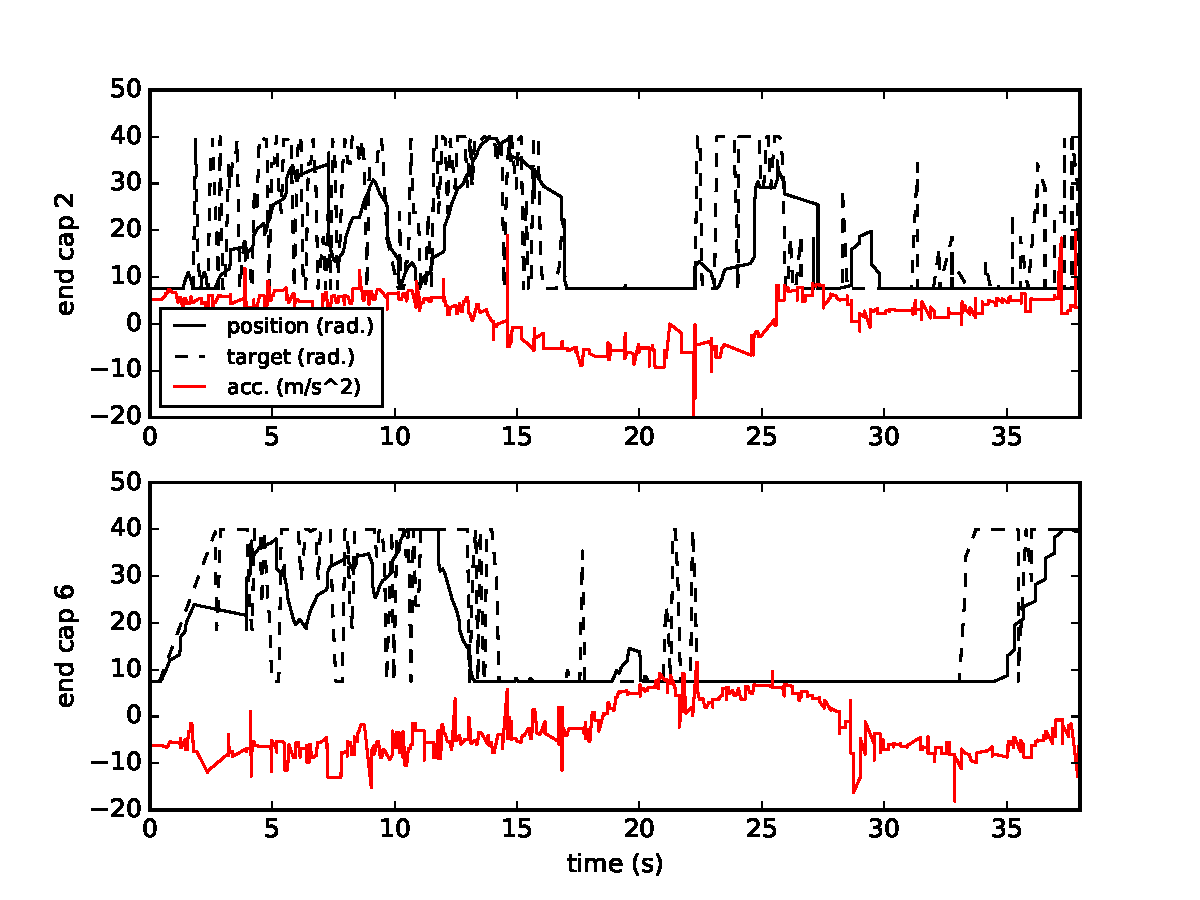
\includegraphics[width=\linewidth]{tex/img/plot_motor}
    \caption{
        \label{fig:commands}
        This plot shows actual motor positions, target motor positions, and 
        single axis accelerometer data over the first 40 seconds of a trial
        for two rod ends which are not connected via cables and not attached
        to the same rod. The commanded positions change based on
        the accelerometer feedback, showing the controller working as the robot
        changes orientation by rolling. The actual motor position  
        lags behind the target motor position due to motor dynamics and network UDP packet loss.
    }
\end{figure}

The open-loop policy was not able to produce any reasonable behavior on the real robot, and we ran it only once due to concerns about hardware safety. 
%The lack
%of performance and safety exhibited by this policy can be explained by viewing
%the difference in motor commands sent by the learned policy in simulation and on
%the real robot, shown in Figure~\ref{fig:commands}. 
% Due to various modeling
% imprecisions, the simulated \SB{} has a greater maximum motor velocity, and the
% policy uses this discrepancy to achieve faster locomotion. The open-loop policy
% attempts to mimic this on the real robot, which does not work because the robot
% cannot reach the same motor positions over a fixed number of time steps as in
% simulation. 
%In addition, despite following all of the action constraints, the
%open-loop policy is dangerous for the cables because they are frayed by the
%constant expansion and contraction. 
%and we can see that it
%adopts a strategy that applies motor commands for a longer period of time in
%order to move the robot into the desired configuration and produce a successful
%locomotion gait.

% \section{CPG or Other Controller}
% \label{cpg_controller}

% \section{Dynamic Rolling}
% \label{dyncamic_rolling}